\documentclass[aspectratio=169,10pt]{beamer}

% -------------------------------------------------------
% KAUST Academy Template  --  Python Pathway · Course 1
% -------------------------------------------------------

\usepackage[T1]{fontenc}
\usepackage[utf8]{inputenc}
\usepackage{tikz}
\usetikzlibrary{arrows.meta,positioning,shadows.blur,calc,fit,
                decorations.pathreplacing,shapes.geometric}
\usepackage{array}
\usepackage{tabularx}
\usepackage{booktabs}
\usepackage[most]{tcolorbox}
\usepackage{ragged2e}
\usepackage{adjustbox}
\usepackage{xcolor}
\usepackage{listings}
\usepackage{graphicx}
\usepackage{subcaption}
\usepackage{amsmath,amssymb}
\usepackage{multirow}
\usepackage{multicol}
\usepackage{hyperref}
\hypersetup{colorlinks=true}

% -------------------------------------------------------
% KAUST Stanford Beamer Theme
% (beamerthemeStanford.sty, beamercolorthemestanford.sty,
%  beamerouterthemesimplefooter.sty must be on the TeX path
%  or in the same directory as this file)
% -------------------------------------------------------
\usetheme{Stanford}

\logo{%
  
\includegraphics[height=0.3in]{style_files/kaust_academy_logo.png}\hspace{0.06in}%
  
\includegraphics[height=0.3in]{style_files/LMHLogo_crest.png}%
}

\makeatletter
\let\@@magyar@captionfix\relax
\makeatother

\setbeamertemplate{itemize items}[default]
\setbeamertemplate{itemize subitem}[circle]
\setbeamertemplate{caption}[numbered]
\setbeamertemplate{navigation symbols}{}

% -------------------------------------------------------
% Color Palette  (PrimaryBlue = KAUST Blue RGB 0,51,102)
% -------------------------------------------------------
\definecolor{PrimaryBlue}{RGB}{0,51,102}
\definecolor{LightGray}{RGB}{245,247,250}
\definecolor{LineGray}{RGB}{180,180,180}
\definecolor{CodeGreen}{RGB}{0,118,83}
\definecolor{CodeRed}{RGB}{190,30,30}
\definecolor{CodeBlue}{RGB}{0,55,130}
\definecolor{CodePurple}{RGB}{114,47,145}

% -------------------------------------------------------
% Custom Commands
% -------------------------------------------------------
\newcommand{\blueball}{%
  \tikz[baseline=-0.6ex]\shade[ball color=PrimaryBlue] (0,0) circle (0.065cm);%
}
\setbeamertemplate{itemize item}{\blueball}
\setbeamertemplate{itemize subitem}{\blueball}
\setlength{\leftmargini}{1.1cm}
\setlength{\leftmarginii}{0.8cm}

\newcommand{\keyword}[1]{\textcolor{PrimaryBlue}{\textbf{#1}}}
\newcommand{\myitem}[1]{\item #1\vspace{0.04cm}}

% Numbered-circle helper
\newcommand{\numcircle}[1]{%
  \tikz[baseline=-0.7ex]\node[circle,shade,ball color=PrimaryBlue,
    text=white,font=\scriptsize\bfseries,inner sep=1.2pt,
    minimum size=0.18cm]{#1};%
}
\newenvironment{numberedlines}%
  {\begin{tabular}{@{}p{0.42cm}p{\dimexpr\textwidth-0.75cm\relax}@{}}}%
  {\end{tabular}}
\newcommand{\nline}[2]{\numcircle{#1} & #2 \\[0.13cm]}

% Placeholder badge (for notebook-covered slides)
\newcommand{\placeholderbadge}{%
  \begin{tikzpicture}[remember picture,overlay]
    \node[anchor=north east,fill=orange!18,draw=orange!70!black,
          rounded corners=1mm,inner xsep=2mm,inner ysep=0.8mm,
          font=\scriptsize\bfseries,text=orange!55!black]
      at ([xshift=-0.28cm,yshift=-1.0cm]current page.north east)
      {PLACEHOLDER --- notebook will cover this};
  \end{tikzpicture}%
}

% -------------------------------------------------------
% tcolorbox Styles
% -------------------------------------------------------
\tcbset{
  lecturebox/.style={
    enhanced,
    colback=LightGray,
    colframe=LineGray,
    boxrule=0.35pt,
    arc=2mm,
    left=1.6mm,right=1.6mm,top=0.8mm,bottom=0.8mm,
    drop shadow={black!45!white,opacity=0.35,
                 shadow xshift=1.2mm,shadow yshift=-1.2mm},
    fonttitle=\normalsize,
    coltitle=white,
    colbacktitle=PrimaryBlue,
    boxed title style={arc=2mm,boxrule=0pt},
    attach boxed title to top left={xshift=0mm,yshift=-0.5mm},
    boxed title size=title,
  },
  plainbox/.style={
    enhanced,
    colback=LightGray,
    colframe=LineGray,
    boxrule=0.35pt,
    arc=2mm,
    left=1.6mm,right=1.6mm,top=0.8mm,bottom=0.8mm,
  }
}

% -------------------------------------------------------
% Python / Code Listing Styles
% -------------------------------------------------------
\lstdefinestyle{pycode}{
  language=Python,
  basicstyle=\ttfamily\scriptsize,
  columns=fullflexible,keepspaces=true,showstringspaces=false,
  breaklines=true,frame=single,rulecolor=\color{LineGray},
  backgroundcolor=\color{gray!6},
  keywordstyle=\color{CodeBlue}\bfseries,
  stringstyle=\color{CodeRed},
  commentstyle=\color{CodeGreen},
  xleftmargin=0pt,xrightmargin=0pt
}
\lstdefinestyle{pycodesmall}{style=pycode,basicstyle=\ttfamily\tiny}
\lstdefinestyle{pycodelarge}{language=Python,
  basicstyle=\ttfamily\large,columns=fullflexible,
  keepspaces=true,showstringspaces=false,frame=single,
  rulecolor=\color{LineGray},backgroundcolor=\color{gray!6},
  keywordstyle=\color{CodeBlue}\bfseries,
  stringstyle=\color{CodeRed},commentstyle=\color{CodeGreen},
  xleftmargin=0pt,xrightmargin=0pt}
\lstdefinestyle{pycodemedium}{language=Python,
  basicstyle=\ttfamily\normalsize,columns=fullflexible,
  keepspaces=true,showstringspaces=false,frame=single,
  rulecolor=\color{LineGray},backgroundcolor=\color{gray!6},
  keywordstyle=\color{CodeBlue}\bfseries,
  stringstyle=\color{CodeRed},commentstyle=\color{CodeGreen},
  xleftmargin=0pt,xrightmargin=0pt}
\lstdefinestyle{termcode}{basicstyle=\ttfamily\large,
  columns=fullflexible,keepspaces=true,showstringspaces=false,
  frame=single,rulecolor=\color{LineGray},backgroundcolor=\color{gray!6}}
\lstdefinestyle{outcode}{basicstyle=\ttfamily\large,
  columns=fullflexible,keepspaces=true,showstringspaces=false,
  frame=single,rulecolor=\color{LineGray},backgroundcolor=\color{gray!6}}
\lstdefinestyle{pseudo}{basicstyle=\ttfamily\large,
  columns=fullflexible,keepspaces=true,showstringspaces=false,
  frame=single,rulecolor=\color{LineGray},backgroundcolor=\color{gray!6},
  xleftmargin=0pt,xrightmargin=0pt}
\lstdefinestyle{pseudocode}{basicstyle=\ttfamily\large,
  columns=fullflexible,keepspaces=true,showstringspaces=false,
  frame=single,rulecolor=\color{LineGray},backgroundcolor=\color{gray!6}}

% -------------------------------------------------------
% TikZ Diagram Styles
% -------------------------------------------------------
\tikzset{
  flowbox/.style={draw=black!85,rounded corners=2mm,fill=LightGray,
    minimum width=2.15cm,minimum height=0.68cm,align=center,font=\normalsize},
  flowarrow/.style={-{Latex[length=2.5mm,width=2.0mm]},
    line width=0.8pt,draw=PrimaryBlue},
  levelbox/.style={draw=black!70,rounded corners=2mm,fill=LightGray,
    text width=3.65cm,minimum height=1.15cm,align=center,font=\normalsize},
  codebox/.style={draw=black!70,rounded corners=2mm,fill=gray!7,
    text width=3.3cm,minimum height=1.1cm,align=center,font=\normalsize},
  terminator/.style={draw,rounded corners=2.5mm,minimum width=2.4cm,
    minimum height=0.48cm,fill=gray!5,align=center},
  process/.style={draw,rectangle,minimum width=2.3cm,
    minimum height=0.52cm,fill=gray!5,align=center},
  decision/.style={draw,diamond,aspect=2.05,inner sep=1.3pt,
    minimum width=2.75cm,minimum height=1.1cm,fill=gray!5,align=center},
  io/.style={draw,trapezium,trapezium left angle=70,
    trapezium right angle=110,minimum width=2.4cm,
    minimum height=0.55cm,fill=gray!5,align=center},
}

% -------------------------------------------------------
% Presentation Metadata
% -------------------------------------------------------
\title[Introduction to Python]{Introduction to Python}
% \subtitle{AI Specialization $\cdot$ Python Pathway}
\author[KAUST Academy]{%
  \begin{tabular}{c}
    \Large Naeemullah Khan
  \end{tabular}
  \vspace{-3ex}%
}
\institute{%
  \vskip 8pt
  \begin{figure}
    \centering
    
\includegraphics[height=0.5in]{style_files/kaust_logo.png}\qquad
    
\includegraphics[height=0.5in]{style_files/LMHLogo.png}
  \end{figure}
  \vskip 6pt
  KAUST Academy\\[3pt]
  King Abdullah University of Science and Technology\\[3pt]
  Stage~1 $\cdot$ Course~1%
}
\date{\today}

% =====================================================
\begin{document}
% =====================================================

% ------------------------------------------
% Title / Cover Slide  (footer visible, header suppressed)
% ------------------------------------------
\begin{noheadline}
\begin{frame}
\maketitle
\end{frame}
\end{noheadline}


% ============================================================
%  MODULE 1 — FOUNDATIONS OF PROGRAMMING
% ============================================================

\begin{noheadline}
\begin{frame}
\vspace{1.35cm}
\begin{center}
  {\fontsize{30}{36}\selectfont\textbf{Module 1}}\\[0.35cm]
  {\fontsize{25}{30}\selectfont FOUNDATIONS OF PROGRAMMING}\\[0.7cm]
  \tcbox[colback=PrimaryBlue!6,colframe=PrimaryBlue,arc=3mm,boxrule=1pt,left=8mm,right=8mm,top=4mm,bottom=4mm,fontupper=\Large]{Programming, computers, Python, and AI/ML foundations}
\end{center}
\end{frame}
\end{noheadline}


\begin{frame}
\frametitle{Module Content}
{\large In this module, we build the foundation needed to understand programming,
Python tools, notebooks, algorithms, and first Python output programs.}

\vspace{0.20cm}
\scriptsize
\begin{columns}[T,totalwidth=\textwidth]
\begin{column}{0.49\textwidth}
\begin{itemize}\setlength\itemsep{0.08cm}
  \item What programming languages are, and why computers need precise instructions.
  \item Natural, high-level, low-level, and machine language; high-level vs.\ low-level comparison.
  \item Why programming matters in science, engineering, data science, and AI/ML.
  \item How computers execute instructions: input, program, CPU, memory, storage, and output.
  \item Why Python is popular, what it is good for, and how Python code runs.
  \item File types and workflows: \texttt{.py} scripts, bytecode, REPL, and notebooks.
\end{itemize}
\end{column}
\begin{column}{0.49\textwidth}
\begin{itemize}\setlength\itemsep{0.08cm}
  \item Programming environments: interpreter, code editor or IDE, terminal, and notebook environment.
  \item Using Google Colab for most course coding labs and explanations.
  \item First Python program: \texttt{print()}, strings, numbers, \texttt{sep}, \texttt{end}, comments, and docstrings.
  \item Algorithm thinking: correctness, efficiency, clarity, flowcharts, and pseudocode.
  \item Beginner examples: maximum value, searching, sorting, login validation, and Big-O intuition.
  \item Activities: printing patterns, self-introduction program, formatted receipt, and common mistakes.
\end{itemize}
\end{column}
\end{columns}
\end{frame}


\begin{frame}
\frametitle{What Is a Programming Language?}
\vspace{0cm}
\begin{columns}[T,totalwidth=\textwidth]
\begin{column}{0.50\textwidth}
{\normalsize Imagine that you want to give your computer a task. You say:}

\vspace{0.12cm}
\begin{tcolorbox}[colback=gray!8,colframe=black!55,arc=2mm,boxrule=0.35pt,top=1mm,bottom=1mm]
\centering\large ``Hey computer, calculate 5 + 5.''
\end{tcolorbox}

{\normalsize The problem is that the computer does not understand natural human language in the same way we do. The instruction is ambiguous for the machine, so nothing useful happens.}

\vspace{0.12cm}
{\normalsize Instead, we write instructions in a language the computer can follow.}
\end{column}
\begin{column}{0.48\textwidth}
\centering
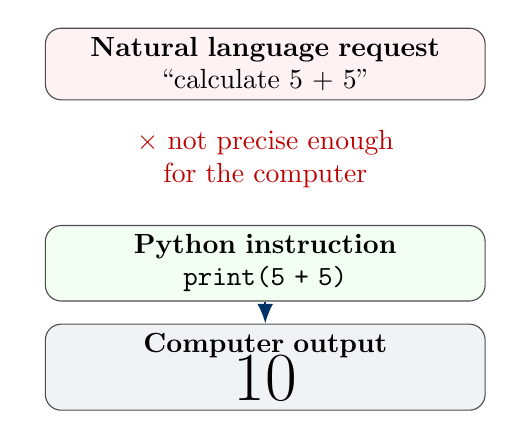
\begin{tikzpicture}[node distance=0.20cm]
  \node[codebox,text width=5.35cm,minimum height=0.75cm,fill=red!5] (natural)
    {\textbf{Natural language request}\\[-0.2mm]``calculate 5 + 5''};
  \node[below=0.25cm of natural,text=red!75!black,text width=5.8cm,
        align=center,font=\normalsize] (cross)
    {$\times$ not precise enough for the computer};
  \node[below=0.35cm of cross,codebox,text width=5.35cm,minimum height=0.75cm,fill=green!5] (code)
    {\textbf{Python instruction}\\[-0.2mm]\texttt{print(5 + 5)}};
  \node[below=0.28cm of code,codebox,text width=5.35cm,minimum height=0.85cm,fill=PrimaryBlue!6] (output)
    {\textbf{Computer output}\\[-0.5mm]{\Huge 10}};
  \draw[flowarrow] (code) -- (output);
\end{tikzpicture}
\end{column}
\end{columns}

\vspace{0.12cm}
\begin{tcolorbox}[enhanced,colback=LightGray,colframe=LineGray,boxrule=0.35pt,arc=2mm,
    left=2mm,right=2mm,top=0.8mm,bottom=0.8mm,
    drop shadow={black!35!white,opacity=0.25,shadow xshift=1mm,shadow yshift=-1mm}]
\small \textcolor{PrimaryBlue}{\textbf{Key idea:}} \keyword{Program} = instructions. \keyword{Programming} = designing and implementing them.
\end{tcolorbox}
\end{frame}


\begin{frame}
\frametitle{From Human Language to Machine Language}
{\small Not all languages are the same. Some are made for people, while others are made for machines.}

\vspace{0.05cm}
\begin{columns}[T,totalwidth=\textwidth]
\begin{column}{0.68\textwidth}
\centering
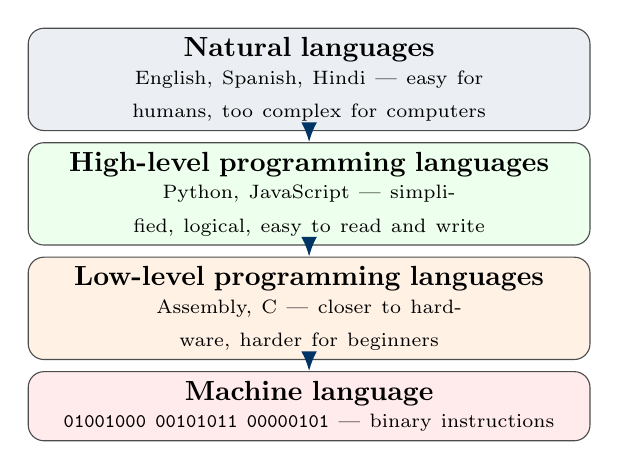
\begin{tikzpicture}[node distance=0.14cm]
  \node[levelbox,text width=6.9cm,minimum height=0.76cm,fill=PrimaryBlue!8] (natural)
    {\textbf{Natural languages}\\[-0.7mm]\scriptsize English, Spanish, Hindi --- easy for humans, too complex for computers};
  \node[levelbox,below=of natural,text width=6.9cm,minimum height=0.76cm,fill=green!7] (high)
    {\textbf{High-level programming languages}\\[-0.7mm]\scriptsize Python, JavaScript --- simplified, logical, easy to read and write};
  \node[levelbox,below=of high,text width=6.9cm,minimum height=0.76cm,fill=orange!10] (low)
    {\textbf{Low-level programming languages}\\[-0.7mm]\scriptsize Assembly, C --- closer to hardware, harder for beginners};
  \node[levelbox,below=of low,text width=6.9cm,minimum height=0.76cm,fill=red!8] (machine)
    {\textbf{Machine language}\\[-0.7mm]\scriptsize \texttt{01001000 00101011 00000101} --- binary instructions};
  \draw[flowarrow] (natural) -- (high);
  \draw[flowarrow] (high) -- (low);
  \draw[flowarrow] (low) -- (machine);
\end{tikzpicture}
\end{column}
\begin{column}{0.30\textwidth}
\begin{tcolorbox}[colback=gray!7,colframe=LineGray,arc=2mm,boxrule=0.35pt,top=0.8mm,bottom=0.8mm]
\textbf{How to read the levels}\vspace{0.03cm}

\scriptsize Each step \textbf{down} brings us closer to how the machine thinks.\\[1mm]
Each step \textbf{up} brings us closer to how humans think.
\end{tcolorbox}

\vspace{0.08cm}
\begin{tcolorbox}[colback=PrimaryBlue!7,colframe=PrimaryBlue,arc=2mm,boxrule=0.4pt,top=0.8mm,bottom=0.8mm]
\scriptsize Python is a high-level bridge: it hides low-level complexity so we can focus on solving the problem.
\end{tcolorbox}
\end{column}
\end{columns}
\end{frame}


\begin{frame}
\frametitle{High-Level vs.\ Low-Level Programming Languages}
\vspace{0cm}
\renewcommand{\arraystretch}{1.18}
\scriptsize
\begin{adjustbox}{max width=\textwidth,max height=6.55cm}
\begin{tabularx}{\textwidth}{>{\bfseries}p{2.55cm} X X}
\toprule
Feature & High-level languages & Low-level languages \\
\midrule
Main idea & Closer to human reasoning and problem solving & Closer to how the hardware actually works \\
Examples & Python, JavaScript, Java, MATLAB & Assembly, C, machine code \\
Ease of reading & Easier to read, write, and learn & Harder to read, write, and debug \\
Control over hardware & Less direct hardware control; many details are hidden & More direct control over memory, registers, and hardware behavior \\
Development speed & Faster for building applications, experiments, and prototypes & Slower because the programmer manages more details \\
Performance focus & Often optimized through libraries and frameworks & Can be highly optimized for speed, memory, or embedded systems \\
Typical uses & Data science, AI/ML, web apps, automation, education, scientific computing & Operating systems, device drivers, embedded systems, microcontrollers, performance-critical code \\
\bottomrule
\end{tabularx}
\end{adjustbox}

\vspace{0.12cm}
\begin{tcolorbox}[lecturebox,title=Remember,top=1mm,bottom=1mm]
\small High-level languages help us express ideas quickly. Low-level languages give more control over the machine, but require more technical detail.
\end{tcolorbox}
\end{frame}


\begin{frame}
\frametitle{Why Programming Matters in Science, Engineering, and AI}
\vspace{0.25cm}
{\large Programming allows us to:}
\vspace{0.15cm}
\begin{itemize}
  \myitem{automate repeated tasks,}
  \myitem{analyze large datasets,}
  \myitem{simulate physical systems,}
  \myitem{build models that learn from data,}
  \myitem{visualize results,}
  \myitem{control robots, sensors, and experiments,}
  \myitem{create reliable and reproducible workflows.}
\end{itemize}

\vspace{0.15cm}
\begin{tcolorbox}[lecturebox,title=AI/ML connection]
Machine learning is not magic. It is a programmed pipeline: load data, clean data, train a model, evaluate results, improve the process, and deploy the solution.
\end{tcolorbox}
\end{frame}


\begin{frame}
\frametitle{A Simple AI/ML Pipeline Is a Program}
\vspace{0.9cm}
\centering
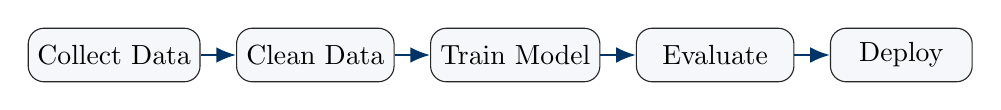
\begin{tikzpicture}[node distance=0.45cm]
  \node[flowbox,minimum width=2.1cm] (collect) {Collect Data};
  \node[flowbox,minimum width=2.0cm,right=of collect] (clean) {Clean Data};
  \node[flowbox,minimum width=2.15cm,right=of clean] (train) {Train Model};
  \node[flowbox,minimum width=2.0cm,right=of train] (eval) {Evaluate};
  \node[flowbox,minimum width=1.8cm,right=of eval] (deploy) {Deploy};
  \draw[flowarrow] (collect) -- (clean);
  \draw[flowarrow] (clean) -- (train);
  \draw[flowarrow] (train) -- (eval);
  \draw[flowarrow] (eval) -- (deploy);
\end{tikzpicture}

\vspace{0.8cm}
\raggedright
{\large Each box is made of many smaller programming tasks:}
\vspace{0.15cm}
\begin{itemize}
  \myitem{reading files, checking errors, filtering rows,}
  \myitem{computing statistics, using libraries,}
  \myitem{saving results, reporting metrics,}
  \myitem{repeating experiments consistently.}
\end{itemize}
\end{frame}


\begin{frame}
\frametitle{How Computers Execute Instructions: The Big Picture}
\vspace{1.1cm}
\centering
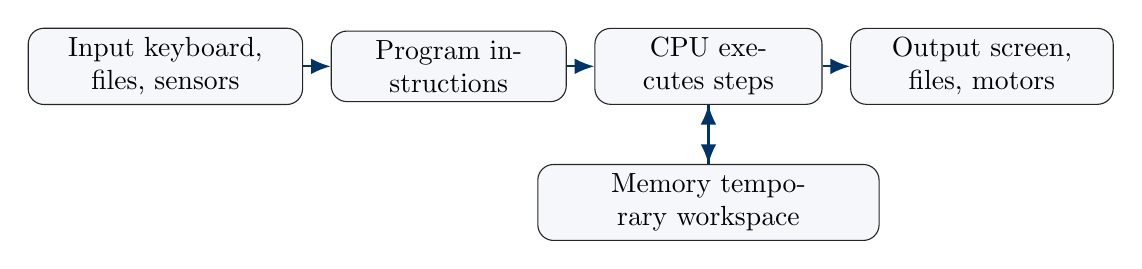
\begin{tikzpicture}[node distance=0.35cm]
  \node[flowbox,text width=3.25cm] (input) {Input keyboard, files, sensors};
  \node[flowbox,text width=2.75cm,right=of input] (program) {Program instructions};
  \node[flowbox,text width=2.65cm,right=of program] (cpu) {CPU executes steps};
  \node[flowbox,text width=3.1cm,right=of cpu] (output) {Output screen, files, motors};
  \node[flowbox,text width=4.1cm,below=0.75cm of cpu] (memory) {Memory temporary workspace};
  \draw[flowarrow] (input) -- (program);
  \draw[flowarrow] (program) -- (cpu);
  \draw[flowarrow] (cpu) -- (output);
  \draw[flowarrow] (cpu) -- (memory);
  \draw[flowarrow] (memory) -- (cpu);
\end{tikzpicture}

\vspace{0.65cm}
\raggedright
\begin{itemize}
  \myitem{The \keyword{CPU} performs operations.}
  \myitem{\keyword{Memory} stores temporary values while the program runs.}
  \myitem{\keyword{Storage} keeps files and programs after power is off.}
  \myitem{\keyword{Input/output} connects the program to the outside world.}
\end{itemize}
\end{frame}


\begin{frame}
\frametitle{CPU, Memory, Storage: A Beginner Analogy}
\vspace{1.0cm}
\small
\renewcommand{\arraystretch}{1.25}
\begin{center}
\begin{tabularx}{0.96\textwidth}{>{\bfseries}p{2.6cm} X X}
\toprule
Computer part & What it does & Analogy \\
\midrule
CPU & Executes instructions step by step & The chef cooking the recipe \\
Memory/RAM & Holds temporary data while the program runs & The kitchen counter \\
Storage & Holds files and programs long term & The pantry or recipe book shelf \\
Program & The instructions to follow & The recipe \\
Input & Data given to the program & Ingredients/orders \\
Output & Result produced by the program & Finished meal/receipt \\
\bottomrule
\end{tabularx}
\end{center}
\end{frame}


\begin{frame}
\frametitle{Why Python Dominates Data Science and AI}
\vspace{0.7cm}
{\large Python is popular in data science and AI because it is:}
\vspace{0.15cm}
\begin{itemize}
  \myitem{readable and beginner-friendly,}
  \myitem{expressive: fewer lines can do more work,}
  \myitem{supported by a huge scientific ecosystem,}
  \myitem{compatible with fast libraries written in C, C++, and Fortran,}
  \myitem{widely used in education, research, startups, and industry.}
\end{itemize}

\vspace{0.15cm}
\begin{tcolorbox}[lecturebox,title=Important libraries you will meet later]
\ttfamily NumPy, Pandas, Matplotlib, Seaborn, scikit-learn, PyTorch, TensorFlow, FastAPI, Jupyter
\end{tcolorbox}
\end{frame}


\begin{frame}
\frametitle{What Python Is Good For}
\vspace{1.1cm}
\begin{columns}[T,totalwidth=\textwidth]
\begin{column}{0.47\textwidth}
\begin{itemize}
  \myitem{Learning programming fundamentals}
  \myitem{Data analysis}
  \myitem{Automation scripts}
  \myitem{Artificial intelligence and machine learning}
  \myitem{Web APIs}
  \myitem{Scientific computing}
\end{itemize}
\end{column}
\begin{column}{0.47\textwidth}
\begin{itemize}
  \myitem{Prototyping ideas quickly}
  \myitem{Reading and writing files}
  \myitem{Visualizing data}
  \myitem{Working with databases}
  \myitem{Connecting to sensors and devices}
  \myitem{Building educational tools}
\end{itemize}
\end{column}
\end{columns}
\end{frame}


\begin{frame}
\frametitle{How Python Works}
\vspace{-0.12cm}
\begin{center}
\begin{adjustbox}{max width=0.94\textwidth}
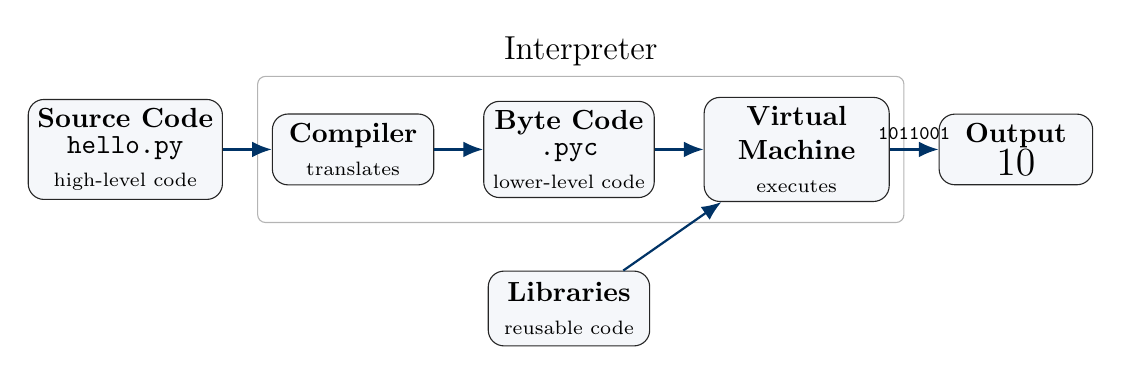
\begin{tikzpicture}[node distance=0.46cm]
  \node[flowbox,minimum width=2.45cm,minimum height=1.20cm] (source)
    {\textbf{Source Code}\\[-1mm]\texttt{hello.py}\\\scriptsize high-level code};
  \node[flowbox,right=0.62cm of source,minimum width=2.05cm] (compiler)
    {\textbf{Compiler}\\\scriptsize translates};
  \node[flowbox,right=0.62cm of compiler,minimum width=2.05cm] (byte)
    {\textbf{Byte Code}\\[-1mm]\texttt{.pyc}\\\scriptsize lower-level code};
  \node[flowbox,right=0.62cm of byte,minimum width=2.35cm] (vm)
    {\textbf{Virtual}\\\textbf{Machine}\\\scriptsize executes};
  \node[flowbox,right=0.62cm of vm,minimum width=1.95cm] (out)
    {\textbf{Output}\\\Large 10};
  \node[draw=LineGray,rounded corners=1mm,fit=(compiler)(byte)(vm),
        inner xsep=0.18cm,inner ysep=0.26cm,
        label={[font=\large]above:Interpreter}] (interpreter) {};
  \node[flowbox,below=0.92cm of byte,minimum width=2.05cm,minimum height=0.95cm] (lib)
    {\textbf{Libraries}\\\scriptsize reusable code};
  \draw[flowarrow] (source) -- (compiler);
  \draw[flowarrow] (compiler) -- (byte);
  \draw[flowarrow] (byte) -- (vm);
  \draw[flowarrow] (vm) -- node[above,font=\scriptsize]{\texttt{1011001}} (out);
  \draw[flowarrow] (lib) -- (vm);
\end{tikzpicture}
\end{adjustbox}
\end{center}
\vspace{-0.02cm}
\begin{itemize}\setlength\itemsep{0.13cm}
  \item We write Python as \keyword{high-level source code} in a file such as \texttt{hello.py}.
  \item Python translates the script into \keyword{byte code}, often stored as a \texttt{.pyc} file.
  \item The \keyword{Python Virtual Machine} executes the byte code and calls libraries when needed.
  \item The final result is the program \keyword{output} that the user sees.
\end{itemize}
\end{frame}


\begin{frame}[fragile]
\frametitle{Python Script vs.\ Byte Code}
\vspace{-0.05cm}
\begin{columns}[T,totalwidth=\textwidth]
\begin{column}{0.49\textwidth}
\textbf{Python script: human-readable source code}
\begin{lstlisting}[style=pycodelarge,basicstyle=\ttfamily\normalsize]
# file name: hello.py
print("Hello from Python")
print(5 + 5)
\end{lstlisting}
\begin{itemize}\setlength\itemsep{0.1cm}
\item Written by the programmer.
\item Easy to read, edit, and share.
\item Saved with the extension \texttt{.py}.
\end{itemize}
\end{column}
\begin{column}{0.49\textwidth}
\textbf{Byte code: machine-oriented instructions}
\begin{lstlisting}[style=termcode,basicstyle=\ttfamily\normalsize]
64 00 5a 00 02 00 65 01
64 01 a6 01 ab 01 01 00
64 02 64 03 7a 00 00 00
\end{lstlisting}
\begin{itemize}\setlength\itemsep{0.1cm}
\item Generated by Python automatically.
\item Not meant to be written by beginners.
\item Often stored in \texttt{\_\_pycache\_\_} as \texttt{.pyc} files.
\end{itemize}
\end{column}
\end{columns}
\begin{tcolorbox}[lecturebox,title=Key idea]
Students write \texttt{.py} files. Python turns them into lower-level byte code so the interpreter can execute them efficiently.
\end{tcolorbox}
\end{frame}


\begin{frame}
\frametitle{Before We Write Python: The Missing Context}
\vspace{-0.05cm}
\begin{tcolorbox}[lecturebox,title=Key idea]
Beginners should not only ask ``What code do I write?'' They should also ask ``Where does this code live, and how does it run?''
\end{tcolorbox}

A Python instruction can be written in different places:
\begin{itemize}\setlength\itemsep{0.13cm}
  \item inside a saved \keyword{script file},
  \item directly into an \keyword{interactive prompt},
  \item inside a \keyword{notebook cell},
  \item through an \keyword{IDE} or cloud environment.
\end{itemize}
\vspace{0.25cm}
\begin{tcolorbox}[lecturebox,title=Checkpoint]
The same Python language can be used through different tools. The tool changes the workflow, not the core language.
\end{tcolorbox}
\end{frame}


\begin{frame}
\frametitle{Two Important File Types: \texttt{.py} and \texttt{.ipynb}}
\vspace{0.45cm}
\renewcommand{\arraystretch}{1.35}
\begin{tabularx}{\textwidth}{>{\bfseries}p{2.25cm}X X}
\toprule
File type & What it contains & Typical use \\
\midrule
\texttt{.py} & Plain Python code saved as a script & Programs, assignments, automation, reusable project files \\
\texttt{.ipynb} & Notebook document containing code cells, text cells, outputs, images, and plots & Data science, AI experiments, teaching, reports, exploration \\
\bottomrule
\end{tabularx}
\vspace{0.55cm}
\begin{tcolorbox}[lecturebox,title=Checkpoint]
Both can contain Python code, but they support different learning and working styles.
\end{tcolorbox}
\end{frame}


\begin{frame}[fragile]
\frametitle{Python Script Files: The \texttt{.py} Workflow}
\vspace{0.4cm}
A \keyword{script} is a saved Python file that can be run again later.
\begin{lstlisting}[style=pycodelarge]
# file name: hello.py
print("Hello from a Python script!")
print("This program can be saved and reused.")
\end{lstlisting}
\vspace{0.2cm}
\begin{tcolorbox}[lecturebox,title=Script workflow]
\begin{enumerate}\setlength\itemsep{0.11cm}
  \item Write code in a file such as \texttt{hello.py}.
  \item Save the file.
  \item Run the file using a terminal or an IDE run button.
  \item Read the output and fix mistakes if needed.
\end{enumerate}
\end{tcolorbox}
\end{frame}


\begin{frame}[fragile]
\frametitle{Running a Script from the Terminal}
\vspace{0.25cm}
If the file is named \texttt{hello.py}, we can run it from a terminal:
\begin{lstlisting}[style=termcode]
python hello.py
\end{lstlisting}
On some systems, the command may be:
\begin{lstlisting}[style=termcode]
python3 hello.py
\end{lstlisting}
\vspace{0.1cm}
\begin{tcolorbox}[lecturebox,title=Beginner interpretation]
This command means: ``Ask the Python interpreter to execute the file named \texttt{hello.py}.''
\end{tcolorbox}
\begin{tcolorbox}[lecturebox,title=Checkpoint]
If the terminal says Python was not found, the issue is usually installation or system path configuration, not your program logic.
\end{tcolorbox}
\end{frame}


\begin{frame}
\frametitle{When Script Files Are Best}
\vspace{0.4cm}
Scripts are best when the goal is to create something \keyword{repeatable}.
\begin{itemize}\setlength\itemsep{0.13cm}
  \item A homework program that should run the same way tomorrow.
  \item A data-cleaning script used on many files.
  \item A small automation task.
  \item A project with multiple Python files.
  \item Code that will be shared through GitHub or submitted for review.
\end{itemize}
\vspace{0.35cm}
\begin{tcolorbox}[lecturebox,title=Important habit]
A script should be readable from top to bottom. Someone else should be able to open the file and understand the order of execution.
\end{tcolorbox}
\end{frame}


\begin{frame}
\frametitle{Interactive Python: The REPL}
\vspace{0.05cm}
\begin{tcolorbox}[lecturebox,title=Key idea]
The REPL is an interactive Python environment where you type one instruction and immediately see the result.
\end{tcolorbox}
\keyword{REPL} stands for:
\begin{itemize}\setlength\itemsep{0.15cm}
  \item \textbf{Read:} Python reads what you typed.
  \item \textbf{Evaluate:} Python computes or executes it.
  \item \textbf{Print:} Python displays the result if there is one.
  \item \textbf{Loop:} Python waits for the next instruction.
\end{itemize}
\vspace{0.25cm}
\begin{tcolorbox}[lecturebox,title=Checkpoint]
The REPL is excellent for quick experiments, but it is not ideal for long programs because the work is not naturally organized as a saved file.
\end{tcolorbox}
\end{frame}


\begin{frame}[fragile]
\frametitle{REPL Example: Immediate Feedback}
\vspace{0.45cm}
A REPL session often shows the prompt \texttt{>>>}.
\begin{lstlisting}[style=termcode,basicstyle=\ttfamily\normalsize]
>>> 2 + 3
5
>>> print("Hello from the REPL")
Hello from the REPL
>>> "AI" + " " + "Python"
'AI Python'
\end{lstlisting}
\vspace{0.3cm}
\begin{tcolorbox}[lecturebox,title=What students should notice]
The REPL is useful for testing tiny ideas before placing them into a larger script or notebook.
\end{tcolorbox}
\end{frame}


\begin{frame}
\frametitle{REPL vs.\ Script: Same Python, Different Workflow}
\vspace{0.65cm}
\renewcommand{\arraystretch}{1.35}
\begin{tabularx}{\textwidth}{>{\bfseries}p{2.4cm}X X}
\toprule
Mode & Strength & Limitation \\
\midrule
REPL & Fast feedback; great for tiny experiments & Not ideal for saving a complete program \\
Script & Organized, reusable, shareable & Slightly slower feedback because you save and run the file \\
\bottomrule
\end{tabularx}
\vspace{0.55cm}
\begin{tcolorbox}[lecturebox,title=Teaching analogy]
The REPL is like trying one sentence aloud. A script is like writing a complete paragraph that can be read again later.
\end{tcolorbox}
\end{frame}


\begin{frame}
\frametitle{Interactive Python Notebook: Code + Explanation + Output}
\vspace{1.0cm}
An \keyword{interactive Python notebook} is an \texttt{.ipynb} document made of cells.
\vspace{0.35cm}
\begin{columns}[T,totalwidth=\textwidth]
\begin{column}{0.49\textwidth}
\begin{tcolorbox}[lecturebox,title=Code cells]
Contain Python code and show output directly below the cell.
\end{tcolorbox}
\end{column}
\begin{column}{0.49\textwidth}
\begin{tcolorbox}[lecturebox,title=Markdown cells]
Contain formatted text, headings, equations, images, and explanations.
\end{tcolorbox}
\end{column}
\end{columns}
\vspace{0.45cm}
\begin{center}
\textbf{This makes notebooks useful for learning, experiments, and AI reports.}
\end{center}
\end{frame}


\begin{frame}
\frametitle{Why Notebooks Are Popular in AI and Data Science}
\vspace{0.25cm}
Notebooks are common in AI/ML because they support an exploratory workflow:
\begin{enumerate}\setlength\itemsep{0.13cm}
  \item Load data.
  \item Inspect a few rows.
  \item Clean or transform the data.
  \item Plot results.
  \item Train or test a model.
  \item Explain observations in text.
\end{enumerate}
\vspace{0.25cm}
\begin{tcolorbox}[lecturebox,title=AI/ML connection]
A notebook can act like a lab notebook: it records not only the code, but also the reasoning, outputs, charts, and intermediate findings.
\end{tcolorbox}
\end{frame}


\begin{frame}
\frametitle{Notebook Execution Order: A Common Beginner Trap}
\vspace{0.05cm}
\begin{tcolorbox}[lecturebox,title=Key idea]
Notebook cells can be run independently, so the order you run them matters.
\end{tcolorbox}
A notebook may look like a document from top to bottom, but the computer remembers what has already been executed.
\begin{itemize}\setlength\itemsep{0.15cm}
  \item Running cell 5 before cell 2 may cause errors.
  \item Changing an earlier cell does not automatically rerun later cells.
  \item Old values can remain in memory and confuse results.
\end{itemize}
\vspace{0.25cm}
\begin{tcolorbox}[lecturebox,title=Checkpoint]
Good notebook habit: when confused, restart the runtime/kernel and run all cells from top to bottom.
\end{tcolorbox}
\end{frame}


\begin{frame}
\frametitle{Programming Environment: What Do You Need?}
\vspace{0.55cm}
To write and run Python, you need:
\vspace{0.12cm}

\begin{numberedlines}
\nline{1}{\keyword{Python interpreter}: the program that executes Python code.}
\nline{2}{\keyword{Code editor or IDE}: where you write code.}
\nline{3}{\keyword{Terminal/command line}: where you can run commands.}
\nline{4}{Optional: \keyword{Notebook environment}: useful for experiments, notes, and data analysis.}
\end{numberedlines}

\vspace{0.22cm}
\begin{tcolorbox}[lecturebox,title=Recommended beginner setup]
Install Python 3, then use VS Code or PyCharm. For data science notebooks, use Jupyter or Google Colab.
\end{tcolorbox}
\end{frame}


\begin{frame}
\frametitle{Common Tools}
\vspace{0.45cm}
\renewcommand{\arraystretch}{1.22}
\begin{tabularx}{\textwidth}{>{\bfseries}p{3.8cm}X}
\toprule
Tool & Purpose \\
\midrule
Python.org installer & Installs the Python interpreter on your computer. \\
VS Code & Lightweight editor with Python extensions. \\
PyCharm & Full Python IDE with strong project tools. \\
Terminal & Runs Python scripts and installation commands. \\
REPL & Interactive Python prompt for quick experiments. \\
Notebook (.ipynb) & Mixes code, text, output, and plots in one document. \\
Google Colab & Cloud notebook environment; useful when local setup is difficult. \\
\bottomrule
\end{tabularx}
\end{frame}


\begin{frame}[fragile]
\frametitle{Checking That Python Works}
\vspace{0.06cm}
In a terminal, try:
\begin{lstlisting}[style=termcode,basicstyle=\ttfamily\normalsize,aboveskip=2pt,belowskip=3pt]
python --version
\end{lstlisting}
\vspace{-0.08cm}
or, on some systems:
\begin{lstlisting}[style=termcode,basicstyle=\ttfamily\normalsize,aboveskip=2pt,belowskip=3pt]
python3 --version
\end{lstlisting}
\vspace{-0.08cm}
Expected output looks like:
\begin{lstlisting}[style=termcode,basicstyle=\ttfamily\normalsize,aboveskip=2pt,belowskip=3pt]
Python 3.12.4
\end{lstlisting}
\vspace{-0.08cm}
\begin{tcolorbox}[lecturebox,title=Checkpoint,top=0.5mm,bottom=0.5mm,fontupper=\normalsize]
If your terminal cannot find Python, the installation path may not be configured.
\end{tcolorbox}
\vspace{-0.08cm}
\begin{tcolorbox}[lecturebox,title=Class demonstration,top=0.5mm,bottom=0.5mm,fontupper=\small]
We will demonstrate Python installation locally, running Python with an IDE, and using the interactive Python REPL.
\end{tcolorbox}
\end{frame}


\begin{frame}
\frametitle{Course Coding Labs: We Will Use Google Colab}
\vspace{0.55cm}
Most of the course coding labs and explanations will be done in \keyword{interactive Python notebooks} using \keyword{Google Colab}.
\vspace{0.22cm}

This is useful because students can focus on learning Python concepts instead of spending too much time on setup problems.
\vspace{0.25cm}
\begin{itemize}\setlength\itemsep{0.13cm}
  \item Code, explanation, and output can live in the same notebook.
  \item Notebooks are easy to share with a link.
  \item Colab runs in the browser and does not require a full local setup.
  \item It is suitable for beginner Python, data science, and later AI/ML work.
\end{itemize}
\vspace{0.3cm}
\begin{tcolorbox}[lecturebox,title=Main message]
Colab will be our main learning environment, while local Python and IDEs are still important professional tools.
\end{tcolorbox}
\end{frame}


\begin{frame}
\frametitle{Google Colab: Cloud Notebooks for Beginners}
\vspace{0.68cm}
\keyword{Google Colab} is a notebook environment that runs in the browser.
\begin{itemize}\setlength\itemsep{0.13cm}
  \item No local Python installation is required.
  \item Code runs on Google's cloud machines.
  \item Notebooks are easy to share with a link.
  \item It supports GPUs and TPUs for later AI workloads.
\end{itemize}
\vspace{0.34cm}
\begin{tcolorbox}[lecturebox,title=Why this matters in Module 1]
Students can begin learning Python immediately without losing time to installation problems.
\end{tcolorbox}
\end{frame}


\begin{frame}
\frametitle{What Actually Happens in Colab?}
\vspace{0.35cm}
When you run a cell in Colab:
\vspace{0.12cm}

\begin{numberedlines}
\nline{1}{Your browser sends the code to a cloud runtime.}
\nline{2}{The runtime executes the Python code.}
\nline{3}{The output is sent back and displayed under the cell.}
\end{numberedlines}

\vspace{0.25cm}
\begin{tcolorbox}[lecturebox,title=Runtime]
A runtime is the temporary machine/session where your code executes. If the runtime disconnects or restarts, variables in memory are lost.
\end{tcolorbox}

\vspace{0.15cm}
\begin{tcolorbox}[lecturebox,title=Checkpoint]
Files and notebooks are not the same as memory. A saved notebook can remain, while runtime variables disappear after restart.
\end{tcolorbox}
\end{frame}


\begin{frame}
\frametitle{Why Colab Is Especially Useful for AI/ML}
\vspace{0.52cm}
Colab fits AI/ML education because it supports later course needs:
\begin{itemize}\setlength\itemsep{0.13cm}
  \item datasets can be uploaded or mounted from Google Drive,
  \item plots and tables appear directly in the notebook,
  \item GPU acceleration can be enabled for deep learning,
  \item notebooks can be shared with instructors or teammates,
  \item examples are easy to reproduce in class.
\end{itemize}
\vspace{0.32cm}
\begin{tcolorbox}[lecturebox,title=Beginner focus]
In the first weeks, Colab is mainly used to remove setup friction. Later, it becomes useful for experiments and model training.
\end{tcolorbox}
\end{frame}


\begin{frame}
\frametitle{Recommended Learning Path for This Course}
\vspace{0.9cm}
\begin{numberedlines}
\nline{1}{Start with \keyword{Google Colab} to avoid setup barriers.}
\nline{2}{Use notebooks to learn concepts, run examples, and document thinking.}
\nline{3}{Practice small \texttt{.py} scripts once basic syntax becomes familiar.}
\nline{4}{Move toward \keyword{VS Code} for larger projects and professional workflows.}
\end{numberedlines}

\vspace{0.25cm}
\begin{tcolorbox}[lecturebox,title=Main principle]
The goal is not to memorize tools. The goal is to understand where code runs and choose the tool that fits the task.
\end{tcolorbox}
\vspace{0.12cm}
\begin{tcolorbox}[lecturebox,title=Class demonstration]
We will demonstrate Google Colab, then write our first Python code using Colab.
\end{tcolorbox}
\end{frame}


\begin{frame}
\frametitle{Notebooks}
\vspace{0.78cm}
A notebook contains cells.
\begin{itemize}\setlength\itemsep{0.14cm}
  \item \keyword{Code cells}: contain Python code and output.
  \item \keyword{Markdown cells}: contain formatted explanation, equations, images, and notes.
\end{itemize}
\vspace{0.28cm}
\begin{tcolorbox}[lecturebox,title=Why notebooks are common in AI/ML]
They combine experiment, explanation, visualization, and results in one place.
\end{tcolorbox}
\vspace{0.18cm}
\begin{tcolorbox}[lecturebox,title=Caution]
Notebook execution order matters. Running cells out of order can confuse beginners.
\end{tcolorbox}
\end{frame}


% ============================================================
%  MODULE 2 — FIRST PROGRAMS, SYNTAX & ALGORITHMIC THINKING
% ============================================================

\begin{noheadline}
\begin{frame}
\vspace{1.35cm}
\begin{center}
  {\fontsize{30}{36}\selectfont\textbf{Module 2}}\\[0.35cm]
  {\fontsize{25}{30}\selectfont First Programs, Syntax \& Algorithmic Thinking}\\[0.7cm]
  \tcbox[colback=PrimaryBlue!6,colframe=PrimaryBlue,arc=3mm,boxrule=1pt,left=8mm,right=8mm,top=4mm,bottom=4mm,fontupper=\Large]{Output programs, syntax rules, and algorithmic thinking}
\end{center}
\end{frame}
\end{noheadline}


\begin{frame}[fragile]
\frametitle{Module Content}
\small
In this module, we will build our first Python programs and develop algorithmic thinking.

\vspace{0.18cm}
\begin{columns}[T,totalwidth=0.96\textwidth]
\begin{column}{0.48\textwidth}
\begin{itemize}\setlength\itemsep{0.05cm}
  \item \keyword{First program}: \texttt{print()}, strings, numbers, \texttt{sep}, \texttt{end}.
  \item \keyword{Comments and docstrings}: single-line and multi-line.
  \item \keyword{Python syntax}: indentation, colons, case sensitivity.
  \item \keyword{Algorithms}: correctness, efficiency, clarity.
\end{itemize}
\end{column}
\begin{column}{0.48\textwidth}
\begin{itemize}\setlength\itemsep{0.05cm}
  \item \keyword{Flowcharts}: symbols, drawing decision flows.
  \item \keyword{Pseudocode}: writing logic without syntax pressure.
  \item \keyword{Small programs}: self-introduction, formatted receipt.
  \item \keyword{Big-O intuition}: a first look at algorithm cost.
\end{itemize}
\end{column}
\end{columns}
\vspace{0.10cm}
\begin{tcolorbox}[lecturebox,title=Learning goal]
Plan before you code: think in algorithms, express in flowcharts or pseudocode, then translate to Python.
\end{tcolorbox}
\end{frame}


\begin{frame}[fragile]
\frametitle{Your First Python Program}
\vspace{0.78cm}
The classic first program prints a message:
\begin{lstlisting}[style=pycodelarge,aboveskip=2pt,belowskip=7pt]
print("Hello, World!")
\end{lstlisting}
What happens?
\vspace{0.12cm}
\begin{numberedlines}
\nline{1}{Python reads the instruction.}
\nline{2}{It recognizes \texttt{print} as a built-in function.}
\nline{3}{It sends the text \texttt{"Hello, World!"} to the screen.}
\end{numberedlines}
\end{frame}


\begin{frame}[fragile]
\frametitle{Understanding \texttt{print()}}
\vspace{0.45cm}
\texttt{print()} displays output.
\begin{lstlisting}[style=pycodelarge,aboveskip=4pt,belowskip=10pt]
print("Python is fun")
print(42)
print("The answer is", 42)
\end{lstlisting}
\begin{tcolorbox}[lecturebox,title=Vocabulary]
\begin{itemize}\setlength\itemsep{0.12cm}
  \item \texttt{print}: function name.
  \item Parentheses \texttt{()}: hold information given to the function.
  \item \texttt{"Python is fun"}: a string, meaning text data.
  \item \texttt{42}: a number.
\end{itemize}
\end{tcolorbox}
\end{frame}


\begin{frame}[fragile]
\frametitle{The \texttt{sep} Parameter}
\vspace{0.43cm}
By default, \texttt{print()} separates multiple values with a space.
\begin{lstlisting}[style=pycodelarge,aboveskip=3pt,belowskip=5pt]
print("A", "B", "C")
print("A", "B", "C", sep="-")
print("2026", "05", "03", sep="/")
\end{lstlisting}
Possible output:
\begin{lstlisting}[style=outcode,aboveskip=3pt,belowskip=7pt]
A B C
A-B-C
2026/05/03
\end{lstlisting}
\keyword{\texttt{sep}} means separator.
\end{frame}


\begin{frame}[fragile]
\frametitle{The \texttt{end} Parameter}
\vspace{0.22cm}
By default, \texttt{print()} ends with a new line.
\begin{lstlisting}[style=pycodelarge,aboveskip=2pt,belowskip=4pt]
print("Hello")
print("World")
\end{lstlisting}
Output:
\begin{lstlisting}[style=outcode,aboveskip=2pt,belowskip=5pt]
Hello
World
\end{lstlisting}
Change the ending:
\begin{lstlisting}[style=pycodelarge,aboveskip=2pt,belowskip=4pt]
print("Hello", end=" ")
print("World")
\end{lstlisting}
Output:
\begin{lstlisting}[style=outcode,aboveskip=2pt,belowskip=2pt]
Hello World
\end{lstlisting}
\end{frame}


\begin{frame}[fragile]
\frametitle{Comments}
\vspace{0.44cm}
Comments are notes for humans. Python ignores them when running the program.
\begin{lstlisting}[style=pycodelarge,aboveskip=3pt,belowskip=7pt]
# This program prints a greeting
print("Welcome to Python") # Display message to user
\end{lstlisting}
Good comments explain why something is done, not only what the code already says.
\vspace{0.12cm}
\begin{tcolorbox}[lecturebox,title=Weak comment,top=0.5mm,bottom=0.5mm]
\texttt{print("Hello") \# prints Hello}
\end{tcolorbox}
\vspace{0.1cm}
\begin{tcolorbox}[lecturebox,title=Better comment,top=0.5mm,bottom=0.5mm]
\texttt{\# First output confirms that the environment is working}
\end{tcolorbox}
\end{frame}


\begin{frame}[fragile]
\frametitle{Docstrings}
\vspace{0.58cm}
A docstring is a special string used to document a module, function, class, or method.\\
You will understand functions more deeply later, but here is an early preview:
\begin{lstlisting}[style=pycodelarge,aboveskip=5pt,belowskip=12pt]
def greet():
    """Display a simple greeting message."""
    print("Hello!")
\end{lstlisting}
\begin{tcolorbox}[lecturebox,title=Beginner takeaway]
Comments and docstrings help people understand code. Good programmers write for both computers and humans.
\end{tcolorbox}
\end{frame}


\begin{frame}[fragile]
\frametitle{Python Syntax: Tiny Details Matter}
\vspace{0.54cm}
Computers are strict. Small syntax details can change meaning or cause errors.
\vspace{0.35cm}
\begin{columns}[T,onlytextwidth]
\begin{column}{0.49\textwidth}
\begin{tcolorbox}[lecturebox,title=Correct]
\begin{lstlisting}[style=pycodelarge,frame=none,backgroundcolor=\color{LightGray},aboveskip=0pt,belowskip=0pt]
print("Hello")
\end{lstlisting}
\end{tcolorbox}
\end{column}
\begin{column}{0.49\textwidth}
\begin{tcolorbox}[lecturebox,title=Incorrect]
\begin{lstlisting}[style=pycodelarge,frame=none,backgroundcolor=\color{LightGray},aboveskip=0pt,belowskip=0pt]
print("Hello"
\end{lstlisting}
\tcblower
Missing closing parenthesis.
\end{tcolorbox}
\end{column}
\end{columns}
\vspace{0.2cm}
\begin{tcolorbox}[lecturebox,title=Checkpoint]
Syntax is the grammar of a programming language. Logic is the meaning of the steps. Both matter.
\end{tcolorbox}
\end{frame}


\begin{frame}
\frametitle{What Is an Algorithm?}
\vspace{0.85cm}
\begin{tcolorbox}[lecturebox,title=Key idea]
An algorithm is a finite, ordered set of steps for solving a problem.
\end{tcolorbox}
\vspace{0.18cm}
A good algorithm should be:
\begin{itemize}\setlength\itemsep{0.13cm}
  \item \keyword{Correct}: it solves the intended problem.
  \item \keyword{Clear}: each step is understandable.
  \item \keyword{Finite}: it eventually stops.
  \item \keyword{Unambiguous}: every step has one clear meaning.
  \item \keyword{Efficient enough}: it does not waste unnecessary time or memory.
\end{itemize}
\end{frame}


\begin{frame}
\frametitle{Algorithm Example: Make Tea}
\vspace{0.25cm}
{\renewcommand{\arraystretch}{0.92}
\begin{numberedlines}
\nline{1}{Put water in kettle.}
\nline{2}{Turn kettle on.}
\nline{3}{Wait until water boils.}
\nline{4}{Put tea bag in cup.}
\nline{5}{Pour hot water into cup.}
\nline{6}{Wait 3 minutes.}
\nline{7}{Remove tea bag.}
\nline{8}{Add sugar if desired.}
\nline{9}{Serve tea.}
\end{numberedlines}}
\vspace{0.02cm}
\begin{tcolorbox}[lecturebox,title=Programming lesson]
Even ordinary tasks have sequence, decisions, and repeated checks.
\end{tcolorbox}
\end{frame}


\begin{frame}
\frametitle{Correctness, Efficiency, and Clarity}
\vspace{1.05cm}
\renewcommand{\arraystretch}{1.36}
\begin{tabularx}{\textwidth}{>{\bfseries}p{3.1cm}X X}
\toprule
Quality & Question to ask & Example \\
\midrule
Correctness & Does it solve the right problem? & Does the login algorithm reject wrong passwords? \\
Efficiency & How much time and memory does it use? & Searching 1 million records should not be painfully slow. \\
Clarity & Can a human understand and maintain it? & Clear step names help others fix or improve the program. \\
\bottomrule
\end{tabularx}
\end{frame}


\begin{frame}
\frametitle{Flowcharts: Visual Algorithms}
\vspace{0.85cm}
\begin{tcolorbox}[lecturebox,title=Key idea]
A flowchart represents the logic of an algorithm using shapes and arrows.
\end{tcolorbox}
\vspace{0.18cm}
Flowcharts are useful because they:
\begin{itemize}\setlength\itemsep{0.14cm}
  \item show the order of steps,
  \item make decisions visible,
  \item reveal loops,
  \item help beginners understand logic before syntax,
  \item support communication between technical and non-technical people.
\end{itemize}
\end{frame}


\begin{frame}
\frametitle{Common Flowchart Symbols}
\vspace{0.65cm}
\begin{center}
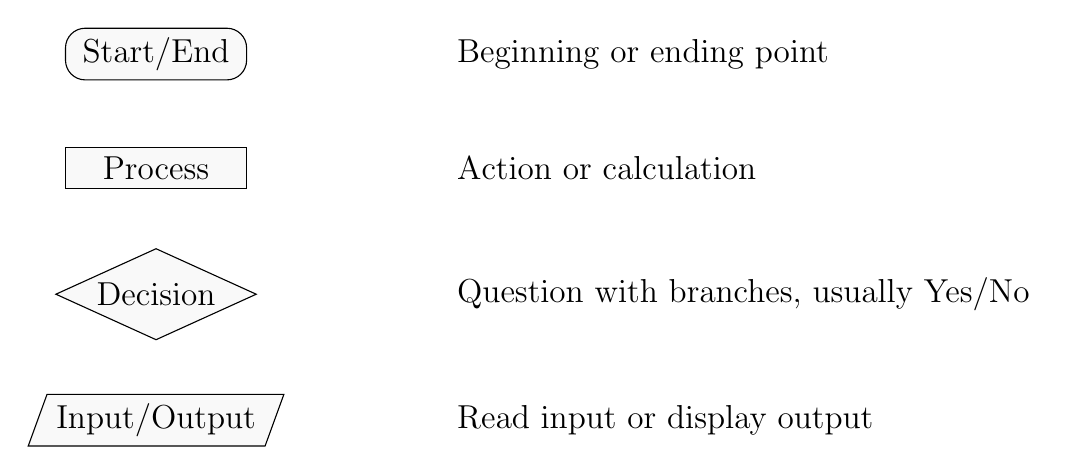
\begin{tikzpicture}[font=\large]
  \node[terminator,minimum width=2.3cm] (start) at (0,0) {Start/End};
  \node[anchor=west] at (3.7,0) {Beginning or ending point};
  \node[process,minimum width=2.3cm] (proc) at (0,-1.45) {Process};
  \node[anchor=west] at (3.7,-1.45) {Action or calculation};
  \node[decision,minimum width=2.55cm] (dec) at (0,-3.05) {Decision};
  \node[anchor=west] at (3.7,-3.05) {Question with branches, usually Yes/No};
  \node[io,minimum width=2.9cm] (inp) at (0,-4.65) {Input/Output};
  \node[anchor=west] at (3.7,-4.65) {Read input or display output};
\end{tikzpicture}
\end{center}
\end{frame}


\begin{frame}
\frametitle{Flowchart Example: Is a Number Positive?}
\vspace{0.12cm}
\begin{center}
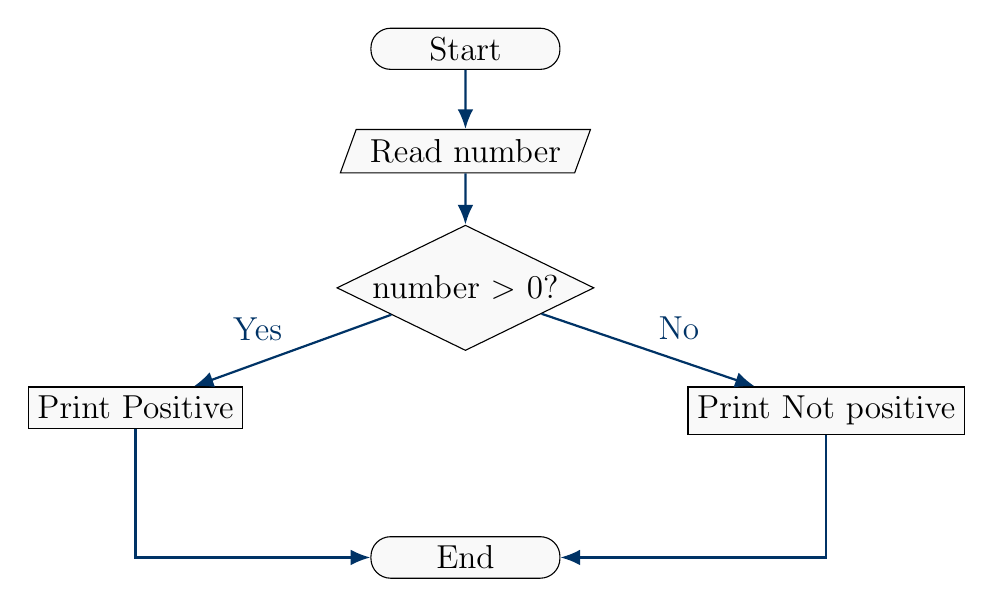
\begin{tikzpicture}[font=\large,node distance=0.75cm]
  \node[terminator] (start) {Start};
  \node[io,below=of start] (read) {Read number};
  \node[decision,below=0.65cm of read] (dec) {number $>$ 0?};
  \node[process,below left=0.85cm and 2.0cm of dec] (pos) {Print Positive};
  \node[process,below right=0.85cm and 2.0cm of dec] (notpos) {Print Not positive};
  \node[terminator,below=2.35cm of dec] (end) {End};
  \draw[flowarrow] (start) -- (read);
  \draw[flowarrow] (read) -- (dec);
  \draw[flowarrow] (dec) -- node[above left,text=PrimaryBlue] {Yes} (pos);
  \draw[flowarrow] (dec) -- node[above right,text=PrimaryBlue] {No} (notpos);
  \draw[flowarrow] (pos) |- (end);
  \draw[flowarrow] (notpos) |- (end);
\end{tikzpicture}
\end{center}
\end{frame}


\begin{frame}
\frametitle{Pseudocode: Code-Like Thinking Without Syntax Pressure}
\vspace{0.85cm}
\begin{tcolorbox}[lecturebox,title=Key idea]
Pseudocode is an informal way to write algorithm steps using human-readable statements.
\end{tcolorbox}
\vspace{0.18cm}
Pseudocode is not real Python. It is a planning tool.
\vspace{0.18cm}
\begin{tcolorbox}[lecturebox,title=Why use pseudocode?]
\begin{itemize}\setlength\itemsep{0.12cm}
  \item It focuses on logic, not punctuation.
  \item It can be understood by people who know different languages.
  \item It helps detect missing steps before coding.
  \item It makes translation into Python easier.
\end{itemize}
\end{tcolorbox}
\end{frame}


\begin{frame}
\frametitle{Pseudocode Example: Positive Number}
\vspace{0.55cm}
\begin{tcolorbox}[colback=gray!6,colframe=LineGray,boxrule=0.35pt,arc=0pt,left=1.5mm,right=1.5mm,top=1.5mm,bottom=1.5mm]
{\ttfamily\large
START\par
READ number\par
IF number is greater than 0 THEN\par
\hspace*{1cm}DISPLAY ``Positive''\par
ELSE\par
\hspace*{1cm}DISPLAY ``Not positive''\par
END IF\par
END\par
}
\end{tcolorbox}
\vspace{0.25cm}
\begin{tcolorbox}[lecturebox,title=Notice]
The pseudocode is structured like code, but it is not tied to any exact programming language syntax.
\end{tcolorbox}
\end{frame}


\begin{frame}
\frametitle{Flowchart vs.\ Pseudocode vs.\ Python}
\vspace{0.85cm}
\renewcommand{\arraystretch}{1.25}
\begin{tabularx}{\textwidth}{>{\bfseries}p{2.8cm}X X}
\toprule
Representation & Best for & Limitation \\
\midrule
Flowchart & Visualizing decisions, branches, loops & Can become large for complex programs \\
Pseudocode & Planning logic in readable steps & Cannot be executed by computer \\
Python code & Running the actual program & Requires correct syntax \\
\bottomrule
\end{tabularx}
\vspace{0.35cm}
A beginner-friendly workflow:
\vspace{0.45cm}
\begin{center}
\Large Problem $\rightarrow$ Algorithm $\rightarrow$ Flowchart $\rightarrow$ Pseudocode $\rightarrow$ Python
\end{center}
\end{frame}


\begin{frame}
\frametitle{Activity: Login Validation Flowchart}
\vspace{0.55cm}
Task: Draw a flowchart for this process.
\vspace{0.18cm}
\begin{numberedlines}
\nline{1}{Start.}
\nline{2}{Ask for username.}
\nline{3}{Ask for password.}
\nline{4}{If username equals the stored username and password equals the stored password, display ``Login successful.''}
\nline{5}{Otherwise, display ``Invalid username or password.''}
\nline{6}{End.}
\end{numberedlines}
\vspace{0.25cm}
\begin{tcolorbox}[lecturebox,title=Challenge]
Add a maximum of 3 attempts. What changes in the flowchart?
\end{tcolorbox}
\end{frame}


\begin{frame}
\frametitle{Login Validation Flowchart}
\vspace{-0.05cm}
\begin{center}
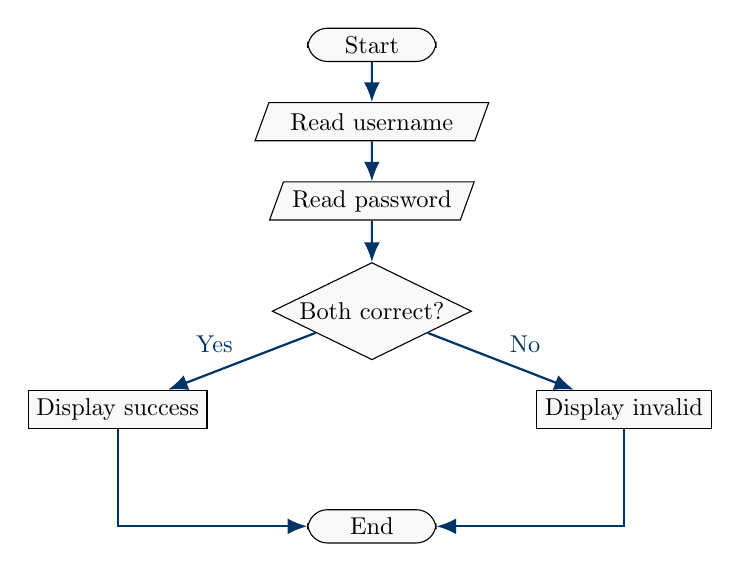
\begin{tikzpicture}[scale=0.88,transform shape,font=\normalsize,node distance=0.58cm]
  \node[terminator,minimum width=1.85cm] (start) {Start};
  \node[io,minimum width=2.45cm,below=of start] (user) {Read username};
  \node[io,minimum width=2.45cm,below=of user] (pass) {Read password};
  \node[decision,minimum width=2.7cm,below=0.60cm of pass] (dec) {Both correct?};
  \node[process,minimum width=2.1cm,below left=0.78cm and 1.65cm of dec] (success) {Display success};
  \node[process,minimum width=2.05cm,below right=0.78cm and 1.65cm of dec] (invalid) {Display invalid};
  \node[terminator,minimum width=1.85cm,below=2.15cm of dec] (end) {End};
  \draw[flowarrow] (start) -- (user);
  \draw[flowarrow] (user) -- (pass);
  \draw[flowarrow] (pass) -- (dec);
  \draw[flowarrow] (dec) -- node[above left,text=PrimaryBlue] {Yes} (success);
  \draw[flowarrow] (dec) -- node[above right,text=PrimaryBlue] {No} (invalid);
  \draw[flowarrow] (success) |- (end);
  \draw[flowarrow] (invalid) |- (end);
\end{tikzpicture}
\end{center}
\end{frame}


\begin{frame}[fragile]
\frametitle{Algorithm Example: Find the Maximum Number}
\vspace{0.18cm}
Problem: Given a list of numbers, find the largest value.
\vspace{0.12cm}
\begin{lstlisting}[style=pseudo,basicstyle=\ttfamily\normalsize]
START
SET largest to first number in list
FOR each remaining number in list
    IF number is greater than largest THEN
        SET largest to number
    END IF
END FOR
DISPLAY largest
END
\end{lstlisting}
\vspace{0.12cm}
\begin{tcolorbox}[lecturebox,title=Important assumption]
The list must contain at least one number. If the list is empty, there is no maximum.
\end{tcolorbox}
\end{frame}


\begin{frame}
\frametitle{Trace Example: Find Maximum}
\vspace{0.72cm}
Input list: \texttt{[4, 9, 2, 11, 5]}
\vspace{0.05cm}
\renewcommand{\arraystretch}{1.1}
\begin{tabularx}{\textwidth}{>{\bfseries}p{1.75cm}p{2.25cm}p{2.55cm}X}
\toprule
Step & Current number & Largest before & Action \\
\midrule
Start & 4 & none & Set largest = 4 \\
1 & 9 & 4 & 9 is greater than 4, set largest = 9 \\
2 & 2 & 9 & 2 is not greater than 9, keep largest = 9 \\
3 & 11 & 9 & 11 is greater than 9, set largest = 11 \\
4 & 5 & 11 & 5 is not greater than 11, keep largest = 11 \\
\bottomrule
\end{tabularx}
\vspace{0.28cm}
Final answer: \texttt{11}
\end{frame}


\begin{frame}[fragile]
\frametitle{Algorithm Example: Search for an Item}
\vspace{0.08cm}
Problem: Determine whether a target item appears in a list.
\vspace{0.08cm}
\begin{lstlisting}[style=pseudo,basicstyle=\ttfamily\normalsize]
START
SET found to False
FOR each item in list
    IF item equals target THEN
        SET found to True
        STOP searching
    END IF
END FOR
IF found is True THEN
    DISPLAY "Item found"
ELSE
    DISPLAY "Item not found"
END IF
END
\end{lstlisting}
\end{frame}


\begin{frame}[fragile]
\frametitle{Algorithm Example: Sorting Numbers Conceptually}
\vspace{0.38cm}
Problem: Put numbers in increasing order.\par
One beginner-friendly idea: repeatedly select the smallest remaining item.
\vspace{0.08cm}
\begin{lstlisting}[style=pseudo,basicstyle=\ttfamily\normalsize]
START
CREATE empty sorted list
WHILE original list is not empty
    FIND smallest number in original list
    REMOVE smallest number from original list
    ADD smallest number to sorted list
END WHILE
DISPLAY sorted list
END
\end{lstlisting}
\vspace{0.10cm}
This is clear, but not always the fastest method for large lists.
\end{frame}


\begin{frame}
\frametitle{Introduction to Big-O: A First Intuition}
\vspace{0.90cm}
\begin{tcolorbox}[lecturebox,title=Key idea]
Big-O notation describes how the work of an algorithm grows as the input size grows.
\end{tcolorbox}
\vspace{0.18cm}
At this stage, do not memorize formulas. Focus on the idea of growth.
\vspace{0.05cm}
\renewcommand{\arraystretch}{1.06}
\begin{tabularx}{\textwidth}{>{\bfseries}p{2.8cm}p{3.45cm}X}
\toprule
Name & Informal meaning & Example intuition \\
\midrule
$O(1)$ & Constant time & Check the first item only \\
$O(n)$ & Linear time & Check every item once \\
$O(n^2)$ & Quadratic time & For every item, compare with every other item \\
$O(\log n)$ & Logarithmic time & Repeatedly cut the problem in half \\
\bottomrule
\end{tabularx}
\end{frame}


\begin{frame}
\frametitle{Big-O Example: Searching a List}
\vspace{0.72cm}
Imagine searching for a name in a list.
\vspace{0.35cm}
\begin{columns}[T,onlytextwidth]
\begin{column}{0.49\textwidth}
\begin{tcolorbox}[lecturebox,title=Unsorted list]
You may need to check every name.\par
Growth pattern: roughly $O(n)$.
\end{tcolorbox}
\end{column}
\begin{column}{0.49\textwidth}
\begin{tcolorbox}[lecturebox,title=Sorted list with smart search]
You can check the middle, discard half, and repeat.\par
Growth pattern: roughly $O(\log n)$.
\end{tcolorbox}
\end{column}
\end{columns}
\vspace{0.42cm}
\begin{tcolorbox}[lecturebox,title=Checkpoint]
Efficiency matters more when data becomes large, which is common in AI and data science.
\end{tcolorbox}
\end{frame}


\begin{frame}[fragile]
\frametitle{Activity: Convert Login Flowchart to Pseudocode}
\vspace{0.40cm}
\begin{lstlisting}[style=pseudo,basicstyle=\ttfamily\small]
START
SET correct_username to "student"
SET correct_password to "python123"
READ username
READ password
IF username equals correct_username AND
   password equals correct_password THEN
    DISPLAY "Login successful"
ELSE
    DISPLAY "Invalid username or password"
END IF
END
\end{lstlisting}
\vspace{0.14cm}
\begin{tcolorbox}[lecturebox,title=Note]
This is still not Python code. It is a clear logic plan.
\end{tcolorbox}
\end{frame}


\begin{frame}[fragile]
\frametitle{From \texttt{print()} to Small Programs}
\vspace{0.55cm}
In the next activities, we will use only \texttt{print()} to create small programs with readable output.
\vspace{0.25cm}
\begin{itemize}
  \item Each line is still one instruction.
  \item Python runs the instructions from top to bottom.
  \item We can use text, spacing, and symbols to make output clearer.
  \item Even simple programs should be organized and easy to read.
\end{itemize}
\vspace{0.42cm}
\begin{tcolorbox}[lecturebox,title=Beginner focus]
Before variables, input, and conditions, we can still practice sequence, output, formatting, and careful program layout.
\end{tcolorbox}
\end{frame}


\begin{frame}[fragile]
\frametitle{Self-Introduction Program}
\vspace{1.45cm}
\begin{lstlisting}[style=pycodelarge]
print("Name: Aisha")
print("Field: Computer Science")
print("Goal: Learn Python for AI")
print("Favorite application: Medical image analysis")
\end{lstlisting}
\vspace{0.42cm}
\begin{tcolorbox}[lecturebox,title=Exercise variation]
Change the values so the program introduces you. Add at least five lines of output.
\end{tcolorbox}
\end{frame}


\begin{frame}[fragile]
\frametitle{Formatted Receipt: First Version}
\vspace{1.05cm}
\begin{lstlisting}[style=pycodemedium]
print("==============================")
print(" PYTHON CAFE")
print("==============================")
print("Item Qty Price")
print("Coffee 2 18.00")
print("Sandwich 1 22.00")
print("------------------------------")
print("Total 40.00")
print("==============================")
\end{lstlisting}
\vspace{0.20cm}
This uses only output statements, but it introduces layout and formatting thinking.
\end{frame}


\begin{frame}[fragile]
\frametitle{Formatted Receipt: Using Escape Characters}
\vspace{0.82cm}
\begin{lstlisting}[style=pycodelarge]
print("Item\tQty\tPrice")
print("Coffee\t2\t18.00")
print("Tea\t1\t8.00")
print("Total\t\t26.00")
\end{lstlisting}
\vspace{0.34cm}
\begin{tcolorbox}[lecturebox,title=Useful escape characters]
\begin{itemize}
  \item \texttt{\textbackslash n}: new line
  \item \texttt{\textbackslash t}: tab space
  \item \texttt{\textbackslash\textbackslash}: backslash character
  \item \texttt{\textbackslash\textquotedbl}: double quote inside a string
\end{itemize}
\end{tcolorbox}
\end{frame}


\begin{frame}[fragile]
\frametitle{Activity 3: Implement Pseudocode Using \texttt{print()}}
\vspace{0.54cm}
Since Module 1 only introduces \texttt{print()}, we can simulate the interaction.
\vspace{0.12cm}
\begin{lstlisting}[style=pycodelarge]
print("Stored username: student")
print("Stored password: python123")
print("User enters username: student")
print("User enters password: python123")
print("Checking username and password...")
print("Login successful")
\end{lstlisting}
\vspace{0.25cm}
\begin{tcolorbox}[lecturebox,title=Why simulate?]
Real input and conditions are introduced in Module 2. For now, focus on sequence and output.
\end{tcolorbox}
\end{frame}


\begin{frame}
\frametitle{Common Beginner Mistakes}
\vspace{0.30cm}
\renewcommand{\arraystretch}{1.18}
\begin{tabularx}{\textwidth}{>{\bfseries}p{2.75cm}p{5.65cm}X}
\toprule
Mistake & Example & Fix \\
\midrule
Skipping planning & Starting code without knowing steps & Write algorithm or pseudocode first \\
Vague instructions & ``Process the data'' & Specify each action \\
Confusing syntax and logic & Correct spelling but wrong steps & Desk-check with examples \\
Ignoring assumptions & Empty list in max algorithm & State assumptions clearly \\
Forgetting quotes & \texttt{print(Hello)} & Use \texttt{print("Hello")} for text \\
Missing parentheses & \texttt{print "Hello"} & Use \texttt{print("Hello")} in Python 3 \\
\bottomrule
\end{tabularx}
\end{frame}


% ============================================================
%  MODULE 3 — VARIABLES, DATA TYPES & INPUT/OUTPUT
% ============================================================

\begin{noheadline}
\begin{frame}
\vspace{1.35cm}
\begin{center}
  {\fontsize{30}{36}\selectfont\textbf{Module 3}}\\[0.35cm]
  {\fontsize{25}{30}\selectfont Variables, Data Types \& Input/Output}\\[0.7cm]
  \tcbox[colback=PrimaryBlue!6,colframe=PrimaryBlue,arc=3mm,boxrule=1pt,left=8mm,right=8mm,top=4mm,bottom=4mm,fontupper=\Large]{Variables, types, casting, and user input}
\end{center}
\end{frame}
\end{noheadline}


\begin{frame}[fragile]
\frametitle{Module Content}
\small
In this module, we will store and work with data using variables, types, and user input.

\vspace{0.18cm}
\begin{columns}[T,totalwidth=0.96\textwidth]
\begin{column}{0.48\textwidth}
\begin{itemize}\setlength\itemsep{0.05cm}
  \item \keyword{Variables}: assignment, naming rules, constants.
  \item \keyword{Data types}: \texttt{int}, \texttt{float}, \texttt{complex}, \texttt{bool}, \texttt{str}, \texttt{NoneType}.
  \item \keyword{Type tools}: \texttt{type()}, \texttt{isinstance()}, and casting.
\end{itemize}
\end{column}
\begin{column}{0.48\textwidth}
\begin{itemize}\setlength\itemsep{0.05cm}
  \item \keyword{Strings and length}: \texttt{len()}, string basics.
  \item \keyword{Input and output}: \texttt{input()}, \texttt{print()}, and f-strings.
  \item \keyword{Type conversion}: changing types with casting functions.
\end{itemize}
\end{column}
\end{columns}
\vspace{0.10cm}
\begin{tcolorbox}[lecturebox,title=Learning goal]
Store data in the right type, convert between types, and interact with the user through input and output.
\end{tcolorbox}
\end{frame}


\begin{frame}[fragile]
\frametitle{Variables: Names for Values}
\begin{tcolorbox}[lecturebox,title=Key idea]
A \keyword{variable} is a name that refers to a value. The value can change as the program runs.
\end{tcolorbox}

\vspace{0.15cm}
\begin{lstlisting}[style=pycode]
student_name = "Aisha"
age = 20
score = 95.5
age = age + 1
\end{lstlisting}

\vspace{0.1cm}
\begin{itemize}
  \myitem{The equal sign \texttt{=} means \keyword{assign the value on the right to the name on the left}.}
  \myitem{Python remembers the latest value assigned to a variable.}
  \myitem{A variable name should help humans understand what the value means.}
\end{itemize}
\end{frame}


\begin{frame}[fragile]
\frametitle{Naming Conventions and Constants}
\begin{columns}[T,totalwidth=\textwidth]
\begin{column}{0.53\textwidth}
\begin{tcolorbox}[lecturebox,title=Good variable names]
Use \keyword{snake\_case}: lowercase words separated by underscores.
\end{tcolorbox}

\begin{lstlisting}[style=pycode]
course_name = "Python"
student_count = 35
final_score = 88
\end{lstlisting}
\end{column}
\begin{column}{0.44\textwidth}
\begin{tcolorbox}[lecturebox,title=Avoid]
\begin{itemize}\setlength\itemsep{0.04cm}
  \item unclear names: \texttt{x}, \texttt{data1}
  \item spaces: \texttt{student count}
  \item starting with a number: \texttt{2score}
\end{itemize}
\end{tcolorbox}
\end{column}
\end{columns}

\vspace{0.2cm}
\begin{tcolorbox}[lecturebox,title=Constants in Python]
Python does not truly lock constants by default. By convention, write values that should not change in uppercase.
\end{tcolorbox}
\begin{lstlisting}[style=pycode]
PI = 3.14159
MAX_ATTEMPTS = 3
\end{lstlisting}
\end{frame}


\begin{frame}[fragile]
\frametitle{Primitive Data Types in One Slide}
\vspace{-0.05cm}
\begin{adjustbox}{max width=\textwidth}
\begin{tabular}{@{}p{2.2cm}p{4.8cm}p{5.4cm}@{}}
\toprule
\textbf{Type} & \textbf{Meaning} & \textbf{Example} \\
\midrule
\texttt{int} & whole number & \texttt{students = 40} \\
\texttt{float} & number with decimal point & \texttt{price = 19.99} \\
\texttt{complex} & number with real and imaginary parts & \texttt{z = 2 + 3j} \\
\texttt{bool} & true/false value & \texttt{is\_ready = True} \\
\texttt{str} & text data & \texttt{name = "Aisha"} \\
\texttt{NoneType} & represents no value yet & \texttt{result = None} \\
\bottomrule
\end{tabular}
\end{adjustbox}

\vspace{0.35cm}
\begin{tcolorbox}[lecturebox,title=Decimal note]
For beginner work, \texttt{float} is enough. For money or exact decimal arithmetic, Python also has \texttt{Decimal} from the \texttt{decimal} module.
\end{tcolorbox}
\end{frame}


\begin{frame}[fragile]
\frametitle{Checking Types: \texttt{type()} and \texttt{isinstance()}}
\begin{tcolorbox}[lecturebox,title=Key idea]
Every value in Python has a type. The type tells Python what operations make sense.
\end{tcolorbox}

\vspace{0.2cm}
\begin{lstlisting}[style=pycode]
age = 20
name = "Aisha"
print(type(age))       # <class 'int'>
print(type(name))      # <class 'str'>
print(isinstance(age, int))   # True
\end{lstlisting}

\vspace{0.15cm}
\begin{itemize}
  \myitem{Use \texttt{type(value)} when you want to inspect what kind of value you have.}
  \myitem{Use \texttt{isinstance(value, type)} when you want a true/false check.}
\end{itemize}
\end{frame}


\begin{frame}[fragile]
\frametitle{Type Conversion: Changing One Type to Another}
\begin{tcolorbox}[lecturebox,title=Key idea]
\keyword{Type conversion} means turning a value from one type into another type.
\end{tcolorbox}

\vspace{0.15cm}
\begin{columns}[T,totalwidth=\textwidth]
\begin{column}{0.49\textwidth}
\textbf{Explicit casting: you ask for it}
\begin{lstlisting}[style=pycode]
age_text = "20"
age = int(age_text)
price = float("19.99")
message = str(100)
flag = bool(1)
\end{lstlisting}
\end{column}
\begin{column}{0.49\textwidth}
\textbf{Implicit conversion: Python handles it}
\begin{lstlisting}[style=pycode]
result = 5 + 2.5
print(result)       # 7.5
print(type(result)) # float
\end{lstlisting}
\end{column}
\end{columns}

\vspace{0.15cm}
\begin{tcolorbox}[lecturebox,title=Checkpoint]
Conversion is useful when input arrives as text, but you need to calculate with numbers.
\end{tcolorbox}
\end{frame}


\begin{frame}[fragile]
\frametitle{Strings and \texttt{len()}}
\begin{tcolorbox}[lecturebox,title=Key idea]
A \keyword{string} is text. Strings are written between quotes.
\end{tcolorbox}

\vspace{0.2cm}
\begin{lstlisting}[style=pycode]
course = "Python Fundamentals"
word = "AI"

print(course)
print(len(course))  # number of characters
print(len(word))    # 2
\end{lstlisting}

\vspace{0.15cm}
\begin{itemize}
  \myitem{\texttt{len(text)} returns how many characters are inside a string.}
  \myitem{Spaces count as characters.}
  \myitem{\texttt{len()} also works with other collections later, such as lists.}
\end{itemize}
\end{frame}


\begin{frame}[fragile]
\frametitle{Printing Values}
\vspace{0.05cm}
\begin{columns}[T,totalwidth=\textwidth]
\begin{column}{0.49\textwidth}
\textbf{Normal \texttt{print()}}
\begin{lstlisting}[style=pycode]
name = "Aisha"
score = 95

print(name)
print("Score:", score)
print("A", "B", "C")
\end{lstlisting}
\end{column}
\begin{column}{0.49\textwidth}
\textbf{Formatted strings: \texttt{f""}}
\begin{lstlisting}[style=pycode]
name = "Aisha"
score = 95

print(f"Student: {name}")
print(f"Score: {score}")
print(f"Next score: {score + 1}")
\end{lstlisting}
\end{column}
\end{columns}

\vspace{0.2cm}
\begin{tcolorbox}[lecturebox,title=Useful options]
\texttt{sep} changes the separator between printed values. \texttt{end} changes what happens at the end of the line.
\end{tcolorbox}
\begin{lstlisting}[style=pycode]
print("2026", "05", "03", sep="/")   # 2026/05/03
print("Hello", end=" "); print("World")
\end{lstlisting}
\end{frame}


\begin{frame}[fragile]
\frametitle{Getting User Input with \texttt{input()}}
\begin{tcolorbox}[lecturebox,title=Key idea]
The \keyword{input()} function pauses the program and waits for the user to type something.
\end{tcolorbox}

\begin{lstlisting}[style=pycode]
name = input("Enter your name: ")
print("Hello", name)
\end{lstlisting}

\begin{itemize}\setlength\itemsep{0.03cm}
  \myitem{The text inside \texttt{input()} is the \keyword{prompt} shown to the user.}
  \myitem{Whatever the user types is stored in the variable.}
  \myitem{By default, \texttt{input()} always gives you a \keyword{string}.}
\end{itemize}

\begin{tcolorbox}[lecturebox,title=Beginner checkpoint]
Even if the user types \texttt{25}, Python receives it as \texttt{"25"}, not as the number \texttt{25}.
\end{tcolorbox}
\end{frame}


\begin{frame}[fragile]
\frametitle{Input and Type Conversion}
When you want to do math with user input, convert it first.

\begin{lstlisting}[style=pycode]
age_text = input("Enter your age: ")
age = int(age_text)
print("Next year you will be", age + 1)
\end{lstlisting}

\begin{columns}[T,totalwidth=\textwidth]
\begin{column}{0.48\textwidth}
\begin{tcolorbox}[lecturebox,title=Useful conversions]
\small
\begin{tabular}{@{}ll@{}}
\texttt{int("42")} & $\rightarrow$ \texttt{42} \\
\texttt{float("3.5")} & $\rightarrow$ \texttt{3.5} \\
\texttt{str(100)} & $\rightarrow$ \texttt{"100"} \\
\texttt{bool(0)} & $\rightarrow$ \texttt{False}
\end{tabular}
\end{tcolorbox}
\end{column}
\begin{column}{0.48\textwidth}
\begin{tcolorbox}[lecturebox,title=Common mistake]
\begin{lstlisting}[style=pycodesmall]
x = input("Number: ")
print(x + 1)   # error: x is text
\end{lstlisting}
\end{tcolorbox}
\end{column}
\end{columns}

\begin{tcolorbox}[lecturebox,title=Rule]
Use \texttt{input()} to collect text. Use \texttt{int()} or \texttt{float()} when you need numbers.
\end{tcolorbox}
\end{frame}


% ============================================================
%  MODULE 4 — OPERATORS, ERRORS & MODULES
% ============================================================

\begin{noheadline}
\begin{frame}
\vspace{1.35cm}
\begin{center}
  {\fontsize{30}{36}\selectfont\textbf{Module 4}}\\[0.35cm]
  {\fontsize{25}{30}\selectfont Operators, Errors \& Modules}\\[0.7cm]
  \tcbox[colback=PrimaryBlue!6,colframe=PrimaryBlue,arc=3mm,boxrule=1pt,left=8mm,right=8mm,top=4mm,bottom=4mm,fontupper=\Large]{Operators, error types, and importing modules}
\end{center}
\end{frame}
\end{noheadline}


\begin{frame}[fragile]
\frametitle{Module Content}
\small
In this module, we will learn to compute with operators, understand errors, and use modules.

\vspace{0.18cm}
\begin{columns}[T,totalwidth=0.96\textwidth]
\begin{column}{0.48\textwidth}
\begin{itemize}\setlength\itemsep{0.05cm}
  \item \keyword{Arithmetic operators}: \texttt{+}, \texttt{-}, \texttt{*}, \texttt{/}, \texttt{//}, \texttt{\%}, \texttt{**}.
  \item \keyword{Comparison operators}: \texttt{==}, \texttt{!=}, \texttt{<}, \texttt{>}, \texttt{<=}, \texttt{>=}.
  \item \keyword{Logical operators}: \texttt{and}, \texttt{or}, \texttt{not}, short-circuit evaluation.
  \item \keyword{Assignment operators}: \texttt{+=}, \texttt{-=}, and compound forms.
\end{itemize}
\end{column}
\begin{column}{0.48\textwidth}
\begin{itemize}\setlength\itemsep{0.05cm}
  \item \keyword{Operator precedence}: order of evaluation, parentheses.
  \item \keyword{Error types}: syntax, runtime, and logic errors; reading tracebacks.
  \item \keyword{Debugging}: print-based debugging strategies.
  \item \keyword{Modules}: importing \texttt{math} and using built-in functions.
\end{itemize}
\end{column}
\end{columns}
\vspace{0.10cm}
\begin{tcolorbox}[lecturebox,title=Learning goal]
Compute correctly, read error messages confidently, and reuse existing Python tools.
\end{tcolorbox}
\end{frame}


\begin{frame}[fragile]
\frametitle{Arithmetic Operators}
\begin{tcolorbox}[lecturebox,title=Key idea]
Arithmetic operators perform mathematical calculations on values.
\end{tcolorbox}

\small
\begin{adjustbox}{max width=\textwidth,max totalheight=0.36\textheight}
\begin{tabular}{@{}p{1.5cm}p{4.1cm}p{5.5cm}@{}}
\toprule
\textbf{Operator} & \textbf{Meaning} & \textbf{Example} \\
\midrule
\texttt{+} & addition & \texttt{5 + 2} gives \texttt{7} \\
\texttt{-} & subtraction & \texttt{5 - 2} gives \texttt{3} \\
\texttt{*} & multiplication & \texttt{5 * 2} gives \texttt{10} \\
\texttt{/} & true division & \texttt{5 / 2} gives \texttt{2.5} \\
\texttt{//} & floor division & \texttt{5 // 2} gives \texttt{2} \\
\texttt{\%} & remainder & \texttt{5 \% 2} gives \texttt{1} \\
\texttt{**} & exponentiation & \texttt{5 ** 2} gives \texttt{25} \\
\bottomrule
\end{tabular}
\end{adjustbox}

\begin{lstlisting}[style=pycodesmall]
minutes = 130
hours = minutes // 60
remaining = minutes % 60
print(hours, "hours and", remaining, "minutes")
\end{lstlisting}
\end{frame}


\begin{frame}[fragile]
\frametitle{Comparison Operators}
\begin{tcolorbox}[lecturebox,title=Key idea]
Comparison operators ask a question and produce a Boolean result: \texttt{True} or \texttt{False}.
\end{tcolorbox}

\small
\begin{adjustbox}{max width=\textwidth,max totalheight=0.35\textheight}
\begin{tabular}{@{}p{1.6cm}p{4.4cm}p{5.3cm}@{}}
\toprule
\textbf{Operator} & \textbf{Meaning} & \textbf{Example} \\
\midrule
\texttt{==} & equal to & \texttt{score == 100} \\
\texttt{!=} & not equal to & \texttt{name != "Ali"} \\
\texttt{<} & less than & \texttt{age < 18} \\
\texttt{>} & greater than & \texttt{temperature > 40} \\
\texttt{<=} & less than or equal to & \texttt{attempts <= 3} \\
\texttt{>=} & greater than or equal to & \texttt{grade >= 60} \\
\bottomrule
\end{tabular}
\end{adjustbox}

\begin{lstlisting}[style=pycodesmall]
score = 75
print(score >= 60)   # True
\end{lstlisting}

{\small \keyword{Important:} Use \texttt{=} for assignment. Use \texttt{==} when asking whether two values are equal.}
\end{frame}


\begin{frame}[fragile]
\frametitle{Logical Operators}
\begin{tcolorbox}[lecturebox,title=Key idea]
Logical operators combine Boolean expressions.
\end{tcolorbox}

\small
\begin{adjustbox}{max width=\textwidth}
\begin{tabular}{@{}p{1.8cm}p{5.1cm}p{5.4cm}@{}}
\toprule
\textbf{Operator} & \textbf{Meaning} & \textbf{Example} \\
\midrule
\texttt{and} & true only if both sides are true & \texttt{age >= 18 and has\_id} \\
\texttt{or} & true if at least one side is true & \texttt{is\_member or has\_coupon} \\
\texttt{not} & reverses the Boolean value & \texttt{not is\_locked} \\
\bottomrule
\end{tabular}
\end{adjustbox}

\begin{lstlisting}[style=pycodesmall]
age = 20
has_id = True
can_enter = age >= 18 and has_id
print(can_enter)
\end{lstlisting}

{\small \keyword{Beginner interpretation:} Read \texttt{age >= 18 and has\_id} as: adult and has ID.}
\end{frame}


\begin{frame}[fragile]
\frametitle{Bitwise Operators: A Light Overview}
\begin{tcolorbox}[lecturebox,title=Key idea]
Bitwise operators work on the binary representation of integers. Beginners only need a high-level awareness for now.
\end{tcolorbox}

\small
\begin{adjustbox}{max width=\textwidth,max totalheight=0.34\textheight}
\begin{tabular}{@{}p{1.6cm}p{3.1cm}p{7.0cm}@{}}
\toprule
\textbf{Operator} & \textbf{Name} & \textbf{Informal meaning} \\
\midrule
\texttt{\&} & bitwise AND & keeps bits that are 1 in both numbers \\
\texttt{|} & bitwise OR & keeps bits that are 1 in either number \\
\texttt{\^{}} & bitwise XOR & keeps bits that are different \\
\texttt{\textasciitilde} & bitwise NOT & flips bits \\
\texttt{<<} & left shift & shifts bits left, often like multiplying by 2 \\
\texttt{>>} & right shift & shifts bits right, often like dividing by 2 \\
\bottomrule
\end{tabular}
\end{adjustbox}

\begin{lstlisting}[style=pycodesmall]
print(5 & 3)   # 1
print(5 | 3)   # 7
\end{lstlisting}

{\small \keyword{Where they appear:} masks, permissions, embedded systems, and low-level code.}
\end{frame}


\begin{frame}[fragile]
\frametitle{Assignment Operators}
\begin{tcolorbox}[lecturebox,title=Key idea]
Assignment operators update variables. They are shortcuts for common update patterns.
\end{tcolorbox}

\small
\begin{adjustbox}{max width=\textwidth,max totalheight=0.44\textheight}
\begin{tabular}{@{}p{1.7cm}p{4.6cm}p{5.9cm}@{}}
\toprule
\textbf{Operator} & \textbf{Meaning} & \textbf{Equivalent form} \\
\midrule
\texttt{=} & assign a value & \texttt{x = 10} \\
\texttt{+=} & add then assign & \texttt{x += 2} means \texttt{x = x + 2} \\
\texttt{-=} & subtract then assign & \texttt{x -= 2} means \texttt{x = x - 2} \\
\texttt{*=} & multiply then assign & \texttt{x *= 2} means \texttt{x = x * 2} \\
\texttt{/=} & divide then assign & \texttt{x /= 2} means \texttt{x = x / 2} \\
\texttt{//=} & floor divide then assign & \texttt{x //= 2} \\
\texttt{**=} & power then assign & \texttt{x **= 2} \\
\texttt{\%=} & remainder then assign & \texttt{x \%= 2} \\
\bottomrule
\end{tabular}
\end{adjustbox}

\begin{lstlisting}[style=pycodesmall]
score = 10
score += 5
print(score)   # 15
\end{lstlisting}
\end{frame}


\begin{frame}[fragile]
\frametitle{Operator Precedence and Associativity}
\begin{tcolorbox}[lecturebox,title=Key idea]
Precedence decides which operator runs first. Associativity decides the direction when operators have the same priority.
\end{tcolorbox}

\begin{columns}[T,totalwidth=\textwidth]
\begin{column}{0.49\textwidth}
\small
\begin{adjustbox}{max width=\textwidth,max totalheight=0.54\textheight}
\begin{tabular}{@{}p{3.0cm}p{3.0cm}@{}}
\toprule
\textbf{Higher first} & \textbf{Examples} \\
\midrule
Parentheses & \texttt{(...)} \\
Power & \texttt{**} \\
Unary signs & \texttt{+x}, \texttt{-x} \\
Multiply/divide & \texttt{* / // \%} \\
Add/subtract & \texttt{+ -} \\
Comparisons & \texttt{== < >=} \\
Logical NOT & \texttt{not} \\
Logical AND & \texttt{and} \\
Logical OR & \texttt{or} \\
\bottomrule
\end{tabular}
\end{adjustbox}
\end{column}
\begin{column}{0.48\textwidth}
\begin{lstlisting}[style=pycodesmall]
result = 2 + 3 * 4
print(result)      # 14

result = (2 + 3) * 4
print(result)      # 20
\end{lstlisting}

\begin{tcolorbox}[lecturebox,title=Best habit]
Use parentheses when they make the expression easier to read, even if Python does not require them.
\end{tcolorbox}
\end{column}
\end{columns}
\end{frame}


\begin{frame}[fragile]
\frametitle{Short-Circuit Evaluation}
\begin{tcolorbox}[lecturebox,title=Key idea]
Python may stop checking a logical expression early if the final answer is already known.
\end{tcolorbox}

\begin{columns}[T,totalwidth=\textwidth]
\begin{column}{0.49\textwidth}
\begin{tcolorbox}[lecturebox,title=With \texttt{and}]
\small
If the first part is \texttt{False}, Python skips the second part.
\begin{lstlisting}[style=pycodesmall]
x = 0
print(x != 0 and 10 / x > 1)
\end{lstlisting}
No division error happens.
\end{tcolorbox}
\end{column}
\begin{column}{0.49\textwidth}
\begin{tcolorbox}[lecturebox,title=With \texttt{or}]
\small
If the first part is \texttt{True}, Python skips the second part.
\begin{lstlisting}[style=pycodesmall]
is_admin = True
print(is_admin or has_permission)
\end{lstlisting}
The second part is unnecessary.
\end{tcolorbox}
\end{column}
\end{columns}

\begin{tcolorbox}[lecturebox,title=Why it matters]
\small Short-circuiting helps write safe checks and avoid unnecessary work.
\end{tcolorbox}
\end{frame}


\begin{frame}[fragile]
\frametitle{Calling Built-in Functions}
\begin{tcolorbox}[lecturebox,title=Key idea]
A \keyword{function call} asks Python to run a ready-made tool and return a result.
\end{tcolorbox}

\begin{lstlisting}[style=pycode]
print(abs(-7))             # 7
print(max(4, 9, 2))        # 9
print(min(4, 9, 2))        # 2
print(round(3.14159, 2))   # 3.14
\end{lstlisting}

\begin{itemize}\setlength\itemsep{0.03cm}
  \myitem{The function name comes first: \texttt{abs}, \texttt{max}, \texttt{min}, \texttt{round}.}
  \myitem{Parentheses hold the \keyword{arguments}: the values given to the function.}
  \myitem{Some functions need one argument; others can use many.}
\end{itemize}

\begin{tcolorbox}[lecturebox,title=Beginner checkpoint]
A function call has the shape \texttt{name(arguments)}. Later, you will learn how to create your own functions.
\end{tcolorbox}
\end{frame}


\begin{frame}[fragile]
\frametitle{Types of Errors: The Big Picture}
\begin{tcolorbox}[lecturebox,title=Key idea]
Errors are normal. Python uses error messages to tell you what went wrong and where to start looking.
\end{tcolorbox}

\small
\begin{adjustbox}{max width=\textwidth,max totalheight=0.42\textheight}
\begin{tabular}{@{}p{3.0cm}p{5.5cm}p{4.6cm}@{}}
\toprule
\textbf{Kind of problem} & \textbf{Meaning} & \textbf{Common Python examples} \\
\midrule
\textbf{Syntax error} & The code breaks Python grammar rules. & \texttt{SyntaxError} \\
\textbf{Runtime error} & The code starts running, then fails. & \texttt{NameError}, \texttt{TypeError}, \texttt{ValueError}, \texttt{ZeroDivisionError}, \texttt{IndexError} \\
\textbf{Logic error} & The code runs, but the answer is wrong. & Wrong formula, wrong condition, wrong order of steps \\
\bottomrule
\end{tabular}
\end{adjustbox}

\begin{lstlisting}[style=pycodesmall]
print("Hello"        # SyntaxError: missing closing parenthesis
print(total)          # NameError if total was never created
print(10 / 0)         # ZeroDivisionError
\end{lstlisting}

\vspace{0.05cm}
{\small \keyword{Course focus:} Do not memorize every error name. Learn to notice the category and read the message calmly.}
\end{frame}


\begin{frame}[fragile]
\frametitle{Reading Tracebacks}
A \keyword{traceback} is Python's report of an error. It usually tells you the file, line number, error type, and message.

\begin{lstlisting}[style=pycodesmall]
Traceback (most recent call last):
  File "main.py", line 2, in <module>
    age = int("twenty")
ValueError: invalid literal for int() with base 10: 'twenty'
\end{lstlisting}

\begin{tcolorbox}[lecturebox,title=How to read it]
\begin{enumerate}\small\setlength\itemsep{0.04cm}
  \item Start near the \keyword{bottom}: \texttt{ValueError} tells you the type of problem.
  \item Look at the \keyword{line number}: line 2 is where Python noticed the error.
  \item Read the message: \texttt{"twenty"} cannot be converted to an integer.
\end{enumerate}
\end{tcolorbox}

\begin{tcolorbox}[lecturebox,title=Beginner habit]
Do not panic when a traceback looks long. Find the last line, then check the line of code it points to.
\end{tcolorbox}
\end{frame}


\begin{frame}[fragile]
\frametitle{Print-Based Debugging}
\begin{tcolorbox}[lecturebox,title=Key idea]
\keyword{Debugging} means finding and fixing mistakes. The simplest debugging tool is \texttt{print()}.
\end{tcolorbox}

\begin{lstlisting}[style=pycode]
price = 50
quantity = 3
print("DEBUG price:", price)
print("DEBUG quantity:", quantity)

total = price * quantity
print("DEBUG total:", total)
\end{lstlisting}

\begin{itemize}\setlength\itemsep{0.03cm}
  \myitem{Print important variables before and after a calculation.}
  \myitem{Use clear labels like \texttt{"DEBUG total:"}.}
  \myitem{Remove or comment out debug prints after fixing the problem.}
\end{itemize}

\vspace{0.05cm}
{\small \keyword{When it helps:} checking variable values, sequence, and whether a line actually runs.}
\end{frame}


\begin{frame}[fragile]
\frametitle{Python Modules: Reusing Existing Tools}
\begin{tcolorbox}[lecturebox,title=Key idea]
A \keyword{module} is a file or library that contains Python code we can reuse instead of writing everything ourselves.
\end{tcolorbox}

\begin{lstlisting}[style=pycode]
import math

print(math.sqrt(25))
print(math.pi)
\end{lstlisting}

\begin{itemize}\setlength\itemsep{0.01cm}
  \myitem{Python already includes many useful modules.}
  \myitem{Use \texttt{import} to bring a module into your program.}
  \myitem{Use \texttt{module.function()} to call tools from that module.}
\end{itemize}

\begin{tcolorbox}[lecturebox,title=Beginner interpretation]
\texttt{math.sqrt(25)} means: use the \texttt{sqrt} function that lives inside the \texttt{math} module.
\end{tcolorbox}
\end{frame}


\begin{frame}[fragile]
\frametitle{The \texttt{math} Library: A First Example}
The \texttt{math} module gives us common mathematical functions and constants.

\begin{columns}[T,totalwidth=\textwidth]
\begin{column}{0.49\textwidth}
\begin{lstlisting}[style=pycode]
import math

radius = 3
area = math.pi * radius ** 2

print(area)
print(round(area, 2))
\end{lstlisting}
\end{column}
\begin{column}{0.48\textwidth}
\begin{tcolorbox}[lecturebox,title=Examples you may see]
\small
\begin{tabular}{@{}ll@{}}
\texttt{math.pi} & $\pi$ value \\
\texttt{math.sqrt(x)} & square root \\
\texttt{math.floor(x)} & round down \\
\texttt{math.ceil(x)} & round up \\
\texttt{math.sin(x)} & sine function
\end{tabular}
\end{tcolorbox}
\end{column}
\end{columns}

\begin{tcolorbox}[lecturebox,title=Important note]
Some simple functions, such as \texttt{round()}, \texttt{min()}, \texttt{max()}, and \texttt{abs()}, are built in. You can use them without importing \texttt{math}.
\end{tcolorbox}
\end{frame}


% ============================================================
%  MODULE 5 — CONDITIONALS & LOOPS
% ============================================================

\begin{noheadline}
\begin{frame}
\vspace{1.35cm}
\begin{center}
  {\fontsize{30}{36}\selectfont\textbf{Module 5}}\\[0.35cm]
  {\fontsize{25}{30}\selectfont Conditionals \& Loops}\\[0.7cm]
  \tcbox[colback=PrimaryBlue!6,colframe=PrimaryBlue,arc=3mm,boxrule=1pt,left=8mm,right=8mm,top=4mm,bottom=4mm,fontupper=\Large]{If/elif/else decisions and for/while repetition}
\end{center}
\end{frame}
\end{noheadline}


\begin{frame}[fragile]
\frametitle{Module Content}
\small
In this module, we will write programs that make decisions and repeat steps.

\vspace{0.18cm}
\begin{columns}[T,totalwidth=0.96\textwidth]
\begin{column}{0.48\textwidth}
\begin{itemize}\setlength\itemsep{0.05cm}
  \item \keyword{Conditionals}: \texttt{if}, \texttt{elif}, \texttt{else}; nested conditionals.
  \item \keyword{Truthiness and falsiness}: what Python treats as true or false.
  \item \keyword{Ternary expressions}: one-line conditional values.
  \item \keyword{Input validation}: checking user input with \texttt{if}.
\end{itemize}
\end{column}
\begin{column}{0.48\textwidth}
\begin{itemize}\setlength\itemsep{0.05cm}
  \item \keyword{For loops}: iterating over sequences and \texttt{range()}.
  \item \keyword{While loops}: condition-controlled repetition.
  \item \keyword{Loop control}: \texttt{break}, \texttt{continue}, \texttt{pass}, \texttt{else}.
  \item \keyword{Loop patterns}: accumulation, search, nested loops, anti-patterns.
\end{itemize}
\end{column}
\end{columns}
\vspace{0.10cm}
\begin{tcolorbox}[lecturebox,title=Learning goal]
Write programs that choose paths and repeat work --- the two most powerful tools in programming.
\end{tcolorbox}
\end{frame}


\begin{frame}[fragile]
\frametitle{Why Programs Need Decisions}
\begin{tcolorbox}[lecturebox,title=Key idea]
A program often needs to choose an action based on data, input, or a situation.
\end{tcolorbox}

\begin{columns}[T,totalwidth=\textwidth]
\begin{column}{0.48\textwidth}
\begin{itemize}\setlength\itemsep{0.04cm}
  \myitem{Is the temperature safe?}
  \myitem{Did the user enter a valid number?}
  \myitem{Is the score high enough to pass?}
  \myitem{Should the program show an error message?}
\end{itemize}
\end{column}
\begin{column}{0.48\textwidth}
\begin{lstlisting}[style=pycode]
temperature = 38

if temperature > 37.5:
    print("Fever warning")
\end{lstlisting}
\end{column}
\end{columns}

\begin{tcolorbox}[lecturebox,title=Programming lesson]
An \texttt{if} statement is how we turn a question into a decision the computer can execute.
\end{tcolorbox}
\end{frame}


\begin{frame}[fragile]
\frametitle{The Basic \texttt{if} Structure}
A simple \texttt{if} statement runs a block only when the condition is true.

\begin{lstlisting}[style=pycode]
floor = 20
actual_floor = floor

if floor > 13:
    actual_floor = floor - 1

print(actual_floor)
\end{lstlisting}

\begin{itemize}\setlength\itemsep{0.02cm}
  \myitem{The header ends with a colon \texttt{:}.}
  \myitem{The indented lines are the block controlled by the \texttt{if}.}
  \myitem{If the condition is false, the block is skipped.}
\end{itemize}

\begin{tcolorbox}[lecturebox,title=Beginner habit]
Read the condition aloud: ``if floor is greater than 13, subtract 1 from it.''
\end{tcolorbox}
\end{frame}


\begin{frame}[fragile]
\frametitle{Choosing Between Two Paths: \texttt{if} and \texttt{else}}
\begin{tcolorbox}[lecturebox,title=Key idea]
Use \texttt{else} when the program should do one thing if the condition is true and another thing otherwise.
\end{tcolorbox}

\begin{lstlisting}[style=pycode]
floor = int(input("Floor: "))

if floor > 13:
    actual_floor = floor - 1
else:
    actual_floor = floor

print("Actual floor:", actual_floor)
\end{lstlisting}

\begin{tcolorbox}[lecturebox,title=Flow of control]
Only one branch runs: either the \texttt{if} branch or the \texttt{else} branch.
\end{tcolorbox}
\end{frame}


\begin{frame}[fragile]
\frametitle{Multiple Alternatives: \texttt{if}, \texttt{elif}, \texttt{else}}
When there are more than two possible outcomes, use \texttt{elif}.

\begin{lstlisting}[style=pycodesmall]
score = 82

if score >= 90:
    print("Excellent")
elif score >= 70:
    print("Passed")
elif score >= 50:
    print("Needs practice")
else:
    print("Try again")
\end{lstlisting}

\begin{itemize}\setlength\itemsep{0cm}
  \myitem{Python checks the branches from top to bottom.}
  \myitem{As soon as one condition is true, that branch runs.}
  \myitem{The remaining branches are skipped.}
\end{itemize}
\end{frame}


\begin{frame}[fragile]
\frametitle{Order Matters in \texttt{elif} Chains}
\begin{tcolorbox}[lecturebox,title=Key idea]
Put the more specific or larger cutoff conditions first when using \texttt{elif}.
\end{tcolorbox}

\begin{columns}[T,totalwidth=\textwidth]
\begin{column}{0.49\textwidth}
\begin{tcolorbox}[lecturebox,title=Correct order]
\begin{lstlisting}[style=pycodesmall]
richter = 7.1

if richter >= 8.0:
    print("Severe")
elif richter >= 7.0:
    print("Major")
elif richter >= 4.5:
    print("Light")
\end{lstlisting}
\end{tcolorbox}
\end{column}
\begin{column}{0.49\textwidth}
\begin{tcolorbox}[lecturebox,title=Wrong order]
\begin{lstlisting}[style=pycodesmall]
richter = 7.1

if richter >= 4.5:
    print("Light")
elif richter >= 7.0:
    print("Major")
\end{lstlisting}
\end{tcolorbox}
\end{column}
\end{columns}

\textbf{What happens?} In the wrong order, \texttt{7.1 >= 4.5} is already true, so Python never reaches the stronger category.
\end{frame}


\begin{frame}[fragile]
\frametitle{Nested Conditionals and Readability}
A \keyword{nested conditional} is an \texttt{if} statement inside another \texttt{if} statement.

\begin{columns}[T,totalwidth=\textwidth]
\begin{column}{0.49\textwidth}
\begin{tcolorbox}[lecturebox,title=Nested version]
\begin{lstlisting}[style=pycodesmall]
if age >= 18:
    if has_id:
        print("Allowed")
    else:
        print("Need ID")
else:
    print("Too young")
\end{lstlisting}
\end{tcolorbox}
\end{column}
\begin{column}{0.49\textwidth}
\begin{tcolorbox}[lecturebox,title=Flatter version]
\begin{lstlisting}[style=pycodesmall]
if age < 18:
    print("Too young")
elif not has_id:
    print("Need ID")
else:
    print("Allowed")
\end{lstlisting}
\end{tcolorbox}
\end{column}
\end{columns}

\begin{tcolorbox}[lecturebox,title=Beginner guideline]
Nested conditionals are useful, but too many levels make code hard to read. Prefer simple branches when possible.
\end{tcolorbox}
\end{frame}


\begin{frame}[fragile]
\frametitle{Truthiness and Falsiness}
\begin{tcolorbox}[lecturebox,title=Key idea]
In Python, some values behave like \texttt{False} when used in a condition. This is called \keyword{falsiness}.
\end{tcolorbox}

\begin{columns}[T,totalwidth=\textwidth]
\begin{column}{0.48\textwidth}
\begin{tcolorbox}[lecturebox,title=Common falsy values]
\small
\begin{itemize}\setlength\itemsep{0.03cm}
  \item \texttt{False}
  \item \texttt{None}
  \item \texttt{0}, \texttt{0.0}
  \item \texttt{""} empty string
  \item \texttt{[]} empty list
\end{itemize}
\end{tcolorbox}
\end{column}
\begin{column}{0.49\textwidth}
\begin{lstlisting}[style=pycode]
name = ""

if name:
    print("Name exists")
else:
    print("No name entered")
\end{lstlisting}
\end{column}
\end{columns}

\begin{tcolorbox}[lecturebox,title=Rule of thumb]
Empty or missing values are usually falsy. Non-empty values are usually truthy.
\end{tcolorbox}
\end{frame}


\begin{frame}[fragile]
\frametitle{Ternary Expressions: Small Decisions in One Line}
\begin{tcolorbox}[lecturebox,title=Key idea]
A \keyword{ternary expression} chooses between two values in one line.
\end{tcolorbox}

\begin{lstlisting}[style=pycode]
age = 20
status = "adult" if age >= 18 else "minor"
print(status)
\end{lstlisting}

The general form is:
\begin{lstlisting}[style=pycode]
value_if_true if condition else value_if_false
\end{lstlisting}

\begin{tcolorbox}[lecturebox,title=When to use it]
Use it for short, simple choices. If the condition becomes long or confusing, use a normal \texttt{if}/\texttt{else} block instead.
\end{tcolorbox}
\end{frame}


\begin{frame}[fragile]
\frametitle{Input Validation with \texttt{if}}
\begin{tcolorbox}[lecturebox,title=Key idea]
Input validation means checking user input before trusting it in calculations or decisions.
\end{tcolorbox}

\begin{lstlisting}[style=pycodesmall]
floor = int(input("Floor: "))

if floor == 13:
    print("Error: there is no 13th floor.")
elif floor <= 0 or floor > 20:
    print("Error: floor must be between 1 and 20.")
else:
    actual_floor = floor
    if floor > 13:
        actual_floor = floor - 1
    print("Actual floor:", actual_floor)
\end{lstlisting}

\begin{tcolorbox}[lecturebox,title=Beginner takeaway]
Use conditions to protect your program from invalid cases before running the main logic.
\end{tcolorbox}
\end{frame}


\begin{frame}[fragile]
\frametitle{Loops: Repeating Work}
\begin{tcolorbox}[lecturebox,title=Key idea]
A \keyword{loop} repeats a block of code. We use loops when the same idea must happen many times.
\end{tcolorbox}

\begin{columns}[T,totalwidth=\textwidth]
\begin{column}{0.49\textwidth}
\begin{itemize}\setlength\itemsep{0.04cm}
  \myitem{Process every item in a list.}
  \myitem{Print numbers from 1 to 10.}
  \myitem{Keep asking until input is valid.}
  \myitem{Repeat calculations until a goal is reached.}
\end{itemize}
\end{column}
\begin{column}{0.48\textwidth}
\begin{lstlisting}[style=pycode]
for number in [1, 2, 3]:
    print(number)
\end{lstlisting}
\begin{tcolorbox}[lecturebox,title=Beginner interpretation]
Do the indented instruction once for each value.
\end{tcolorbox}
\end{column}
\end{columns}
\end{frame}


\begin{frame}[fragile]
\frametitle{The \texttt{for} Loop: Iterating Over Values}
Use a \texttt{for} loop when you already have a sequence, range, or iterable to go through.

\begin{lstlisting}[style=pycode]
fruits = ["apple", "banana", "orange"]

for fruit in fruits:
    print(fruit)
\end{lstlisting}

\begin{tcolorbox}[lecturebox,title=Structure]
\texttt{for variable in iterable:} \quad followed by an indented block.
\end{tcolorbox}

\begin{itemize}\setlength\itemsep{0.03cm}
  \myitem{The variable receives one value at a time.}
  \myitem{The loop body runs once per value.}
  \myitem{This works with lists, strings, ranges, and many other iterable objects.}
\end{itemize}
\end{frame}


\begin{frame}[fragile]
\frametitle{The \texttt{range()} Function: start, stop, step}
\texttt{range()} creates a sequence of integers, often used for count-controlled loops.

\begin{columns}[T,totalwidth=\textwidth]
\begin{column}{0.52\textwidth}
\begin{lstlisting}[style=pycode]
for i in range(5):
    print(i)      # 0, 1, 2, 3, 4

for i in range(1, 6):
    print(i)      # 1, 2, 3, 4, 5

for i in range(1, 10, 2):
    print(i)      # 1, 3, 5, 7, 9
\end{lstlisting}
\end{column}
\begin{column}{0.45\textwidth}
\begin{tcolorbox}[lecturebox,title=Remember]
\scriptsize
\begin{tabular}{@{}ll@{}}
\texttt{range(stop)} & starts at 0 \\
\texttt{range(start, stop)} & stops before \texttt{stop} \\
\texttt{range(start, stop, step)} & jumps by \texttt{step}
\end{tabular}
\end{tcolorbox}
\begin{tcolorbox}[lecturebox,title=Common trap]
The stop value is \textbf{not included}. This is a common source of off-by-one errors.
\end{tcolorbox}
\end{column}
\end{columns}
\end{frame}


\begin{frame}[fragile]
\frametitle{The \texttt{while} Loop: Condition-Controlled Repetition}
Use a \texttt{while} loop when repetition depends on a condition being true.

\begin{lstlisting}[style=pycode]
balance = 10000
year = 0

target = 20000
rate = 0.05

while balance < target:
    year = year + 1
    balance = balance + balance * rate

print("Years:", year)
\end{lstlisting}

\begin{tcolorbox}[lecturebox,title=Loop checklist]
Initialize something before the loop, test a condition, and update something inside the loop so the condition can eventually become false.
\end{tcolorbox}
\end{frame}


\begin{frame}[fragile]
\frametitle{\texttt{for} vs.\ \texttt{while}: Choosing the Right Loop}
\begin{center}
\small
\begin{tabularx}{0.95\textwidth}{>{\bfseries}p{2.5cm}X X}
\toprule
Loop & Best for & Example idea \\
\midrule
\texttt{for} & A known collection or count & For each student, print the grade. \\
\texttt{for} with \texttt{range()} & Repeating a known number of times & Print numbers from 1 to 10. \\
\texttt{while} & Repeating until a condition changes & Keep asking until the password is correct. \\
\bottomrule
\end{tabularx}
\end{center}

\begin{columns}[T,totalwidth=\textwidth]
\begin{column}{0.49\textwidth}
\begin{lstlisting}[style=pycodesmall]
for i in range(3):
    print("Try", i)
\end{lstlisting}
\end{column}
\begin{column}{0.49\textwidth}
\begin{lstlisting}[style=pycodesmall]
password = ""
while password != "python":
    password = input("Password: ")
\end{lstlisting}
\end{column}
\end{columns}
\end{frame}


\begin{frame}[fragile]
\frametitle{Loop Control: \texttt{break}, \texttt{continue}, and \texttt{pass}}
These keywords change what happens inside a loop.

\begin{columns}[T,totalwidth=\textwidth]
\begin{column}{0.33\textwidth}
\begin{tcolorbox}[lecturebox,title={\texttt{break}}]
Exit the loop early.
\begin{lstlisting}[style=pycodesmall]
for n in nums:
    if n < 0:
        break
\end{lstlisting}
\end{tcolorbox}
\end{column}
\begin{column}{0.33\textwidth}
\begin{tcolorbox}[lecturebox,title={\texttt{continue}}]
Skip to the next iteration.
\begin{lstlisting}[style=pycodesmall]
for n in nums:
    if n == 0:
        continue
    print(n)
\end{lstlisting}
\end{tcolorbox}
\end{column}
\begin{column}{0.31\textwidth}
\begin{tcolorbox}[lecturebox,title={\texttt{pass}}]
Do nothing for now.
\begin{lstlisting}[style=pycodesmall]
for n in nums:
    pass
\end{lstlisting}
\end{tcolorbox}
\end{column}
\end{columns}

\begin{tcolorbox}[lecturebox,title=Beginner advice]
Use these sparingly. A clear loop is usually better than a clever loop.
\end{tcolorbox}
\end{frame}


\begin{frame}[fragile]
\frametitle{The \texttt{else} Clause on Loops}
\begin{tcolorbox}[lecturebox,title=Key idea]
A loop \texttt{else} runs only if the loop finishes normally without hitting \texttt{break}.
\end{tcolorbox}

\begin{lstlisting}[style=pycode]
numbers = [2, 4, 6, 8]

for n in numbers:
    if n < 0:
        print("Found a negative number")
        break
else:
    print("No negative numbers found")
\end{lstlisting}

\begin{tcolorbox}[lecturebox,title=Useful pattern]
Loop \texttt{else} is useful for search problems: \textit{if you never found the item, do this final action.}
\end{tcolorbox}
\end{frame}


\begin{frame}[fragile]
\frametitle{Nested Loops: Loops Inside Loops}
A \keyword{nested loop} has one loop inside another loop. This is useful for tables, grids, and pairwise comparisons.

\begin{lstlisting}[style=pycode]
for row in range(1, 4):
    for col in range(1, 4):
        print(row, col)
\end{lstlisting}

\begin{columns}[T,totalwidth=\textwidth]
\begin{column}{0.49\textwidth}
\begin{tcolorbox}[lecturebox,title=Use cases]
\small
\begin{itemize}\setlength\itemsep{0.02cm}
  \item Printing tables
  \item Comparing every pair
  \item Working with rows and columns
\end{itemize}
\end{tcolorbox}
\end{column}
\begin{column}{0.49\textwidth}
\begin{tcolorbox}[lecturebox,title=Performance awareness]
If the outer loop runs 100 times and the inner loop runs 100 times, the body runs 10,000 times.
\end{tcolorbox}
\end{column}
\end{columns}
\end{frame}


\begin{frame}[fragile]
\frametitle{Common Loop Algorithms}
Many programs repeat the same loop patterns with different data.

\begin{columns}[T,totalwidth=\textwidth]
\begin{column}{0.49\textwidth}
\begin{lstlisting}[style=pycodesmall]
values = [3, -2, 7, -1]

total = 0
negatives = 0

for value in values:
    total += value
    if value < 0:
        negatives += 1

print(total)
print(negatives)
\end{lstlisting}
\end{column}
\begin{column}{0.48\textwidth}
\begin{tcolorbox}[lecturebox,title=Patterns to recognize]
\small
\begin{itemize}\setlength\itemsep{0.03cm}
  \item Sum values
  \item Count matches
  \item Search for a value
  \item Find minimum or maximum
  \item Build a new list
\end{itemize}
\end{tcolorbox}
\begin{tcolorbox}[lecturebox,title=Checkpoint]
Before coding, describe the pattern in words: ``go through every value and update something.''
\end{tcolorbox}
\end{column}
\end{columns}
\end{frame}


\begin{frame}[fragile]
\frametitle{Avoiding Loop Anti-Patterns}
\begin{tcolorbox}[lecturebox,title=Common mistake]
Do not modify a list while looping over the same list. It can skip values or produce confusing behavior.
\end{tcolorbox}

\begin{columns}[T,totalwidth=\textwidth]
\begin{column}{0.49\textwidth}
\begin{tcolorbox}[lecturebox,title=Risky]
\begin{lstlisting}[style=pycodesmall]
numbers = [1, 2, 3, 4]

for n in numbers:
    if n % 2 == 0:
        numbers.remove(n)
\end{lstlisting}
\end{tcolorbox}
\end{column}
\begin{column}{0.49\textwidth}
\begin{tcolorbox}[lecturebox,title=Safer]
\begin{lstlisting}[style=pycodesmall]
numbers = [1, 2, 3, 4]

odds = []
for n in numbers:
    if n % 2 != 0:
        odds.append(n)
\end{lstlisting}
\end{tcolorbox}
\end{column}
\end{columns}

\begin{tcolorbox}[lecturebox,title=Rule of thumb]
If you need a changed version of a list, build a new list instead of editing the old one while looping.
\end{tcolorbox}
\end{frame}


\begin{frame}[fragile]
\frametitle{Loop Thinking: Initialization, Condition, Update}
\begin{tcolorbox}[lecturebox,title=Key idea]
Every loop has a rhythm: setup, repeat, update, stop.
\end{tcolorbox}

\begin{columns}[T,totalwidth=\textwidth]
\begin{column}{0.48\textwidth}
\begin{lstlisting}[style=pycode]
count = 1        # initialize

while count <= 5: # condition
    print(count)
    count += 1   # update
\end{lstlisting}
\end{column}
\begin{column}{0.49\textwidth}
\begin{itemize}\setlength\itemsep{0.04cm}
  \myitem{What value do we start with?}
  \myitem{When should the loop continue?}
  \myitem{What changes each repetition?}
  \myitem{How do we know it will stop?}
\end{itemize}
\end{column}
\end{columns}

\begin{tcolorbox}[lecturebox,title=Beginner habit]
Trace a small example by hand. Most loop bugs become easier to see when you write down each step.
\end{tcolorbox}
\end{frame}


% ============================================================
%  THANK YOU
% ============================================================

\begin{frame}
\frametitle{Thank You}
\vspace{0.9cm}
\begin{center}
{\fontsize{34}{40}\selectfont \textbf{Thank you!}}\\[0.45cm]
{\fontsize{18}{22}\selectfont Questions and discussion}
\end{center}
\vspace{0.5cm}
\begin{tcolorbox}[lecturebox,title=Course takeaway]
Python is a tool for clear thinking. Start with an algorithm, express it in code, test it, and improve it.
\end{tcolorbox}
\end{frame}

\end{document}
